\documentclass[11pt]{article}
\usepackage[margin=1in]{geometry}
\usepackage{booktabs}
\usepackage{hyperref}
\usepackage{amsmath}
\usepackage{amssymb}
\usepackage{url}
\usepackage{graphicx}
\usepackage{xcolor}
\usepackage{enumerate}
\usepackage{subcaption}
\usepackage{float}
\usepackage{placeins}

\title{Memo 06: Late-Time Spatial Distribution Checking\\
       for FVCOM-MP Cases a, b, and c}
\author{FVCOM-MP Delaware Test Cases}
\date{May 2026}

\begin{document}
\sloppy
\maketitle

\section*{Purpose}

Memo~05 checked the first ten simulation days after the mass-conservation
correction documented in Memo~04.  This memo extends the same spatial
diagnostics to later model output windows centred on simulation day~30 and
simulation day~90.  The focus is the microplastic tracer (\texttt{mp1}) and
its floc-interaction split (\texttt{mp1\_agg}, \texttt{mp1\_dis}) in cases
\texttt{a}, \texttt{b}, and \texttt{c}.

The practical questions are:
\begin{enumerate}[(1)]
  \item Do cases \texttt{a} and \texttt{b} remain identical at later times?
  \item Does corrected case \texttt{c} continue to show active aggregation and
        bed exchange?
  \item Do the late-time pointwise-maximum maps show isolated numerical
        accumulation artifacts?
  \item Are the aggregated plus disaggregated fields still consistent with
        total \texttt{mp1}?
\end{enumerate}

\section*{Methodology}

The existing Python analysis script was updated to process day-specific MAT
files:
\begin{itemize}
  \item Day~10: \texttt{spatial\_snapshots\_\{a,b,c\}.mat}
  \item Day~30: \texttt{spatial\_snapshots\_\{a,b,c\}\_day30.mat}
  \item Day~90: \texttt{spatial\_snapshots\_\{a,b,c\}\_day90.mat}
\end{itemize}

The outputs are now organized as:
\begin{itemize}
  \item \texttt{PYTHON/output/spatial\_distribution/day10/}
  \item \texttt{PYTHON/output/spatial\_distribution/day30/}
  \item \texttt{PYTHON/output/spatial\_distribution/day90/}
\end{itemize}

For day~30 the spatial snapshot window is simulation days
29.500--29.957 and the station time-series window is simulation days
20.000--29.957.  For day~90 the spatial snapshot window is simulation days
89.500--89.957 and the station time-series window is simulation days
80.000--89.957.  Each day folder also contains a reproducible
\texttt{summary\_stats.csv} file with per-case maxima, means, positive-node
counts, split-consistency errors, and cross-case difference magnitudes.

\section*{Numerical Summary}

\begin{table}[H]
\centering
\caption{Selected day-mean statistics from \texttt{summary\_stats.csv}.
         Positive bed nodes are counted from the day-mean
         \texttt{bot\_mass} field.}
\label{tab:late_summary}
\begin{tabular}{llrrrr}
\toprule
Day & Case & max \texttt{mp1\_davg} & max \texttt{mp1\_agg\_davg}
    & max \texttt{bot\_mass} & positive bed nodes \\
    &      & kg\,m$^{-3}$ & kg\,m$^{-3}$ & kg\,m$^{-2}$ & count \\
\midrule
30 & a & $3.36\times10^{-4}$ & --                 & $0$                 & 0 \\
30 & b & $3.36\times10^{-4}$ & $0$                & $0$                 & 0 \\
30 & c & $4.62\times10^{-3}$ & $1.10\times10^{-3}$& $1.95\times10^{-1}$ & 63\,008 \\
\midrule
90 & a & $2.81\times10^{-4}$ & --                 & $0$                 & 0 \\
90 & b & $2.81\times10^{-4}$ & $0$                & $0$                 & 0 \\
90 & c & $1.49\times10^{-3}$ & $6.46\times10^{-5}$& $2.21\times10^{-3}$ & 68\,351 \\
\bottomrule
\end{tabular}
\end{table}

The \texttt{b-a} differences are exactly zero in the generated summary for
\texttt{mp1\_davg} and \texttt{bot\_mass} at both day~30 and day~90.  Case
\texttt{b} also retains zero aggregated mass and zero bed mass in both
late-time windows.  In case~\texttt{c}, the maximum split-consistency error
$|\texttt{mp1\_agg}+\texttt{mp1\_dis}-\texttt{mp1}|$ is
$4.46\times10^{-10}$~kg\,m$^{-3}$ at day~30 and
$1.14\times10^{-10}$~kg\,m$^{-3}$ at day~90 for the depth-averaged fields.

\section*{Results}

\subsection*{R1. Day-Mean Depth-Averaged mp1: Day 30}

\begin{figure}[H]
\centering
\begin{subfigure}[b]{0.32\textwidth}
  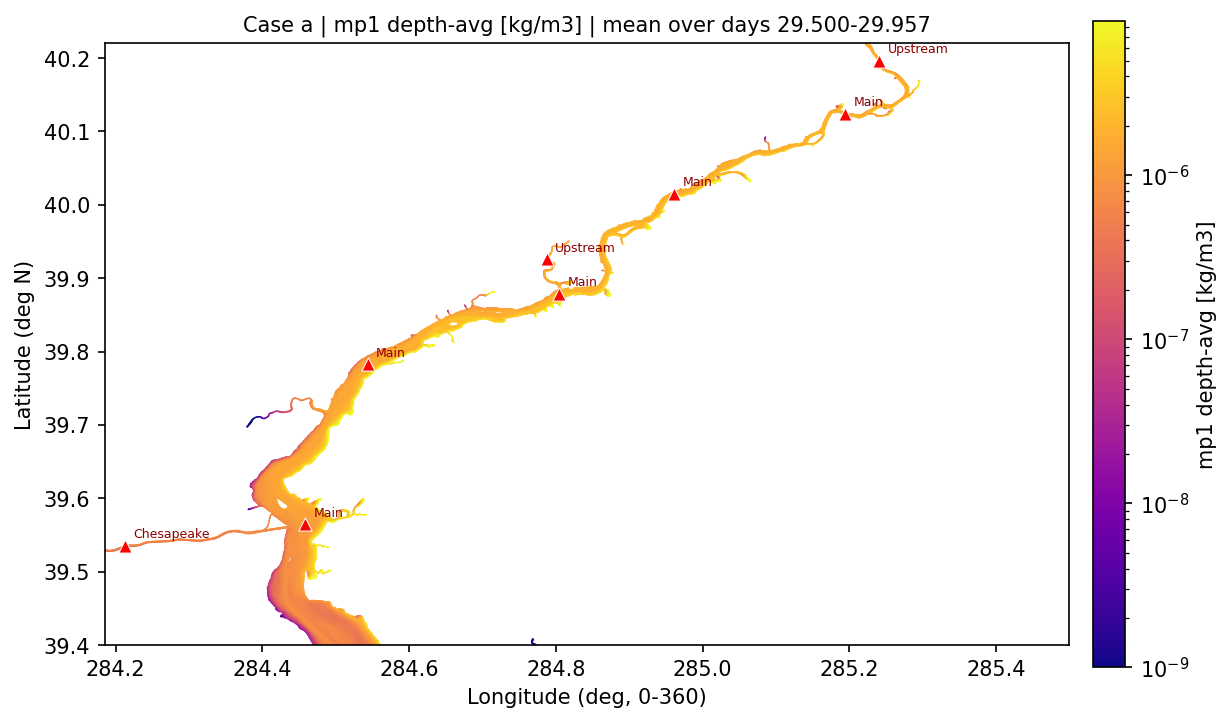
\includegraphics[width=\textwidth]{../FVCOM_MP_test_run/PYTHON/output/spatial_distribution/day30/planview_dayavg_mp1_davg_casea.png}
  \caption{Case a}
\end{subfigure}
\hfill
\begin{subfigure}[b]{0.32\textwidth}
  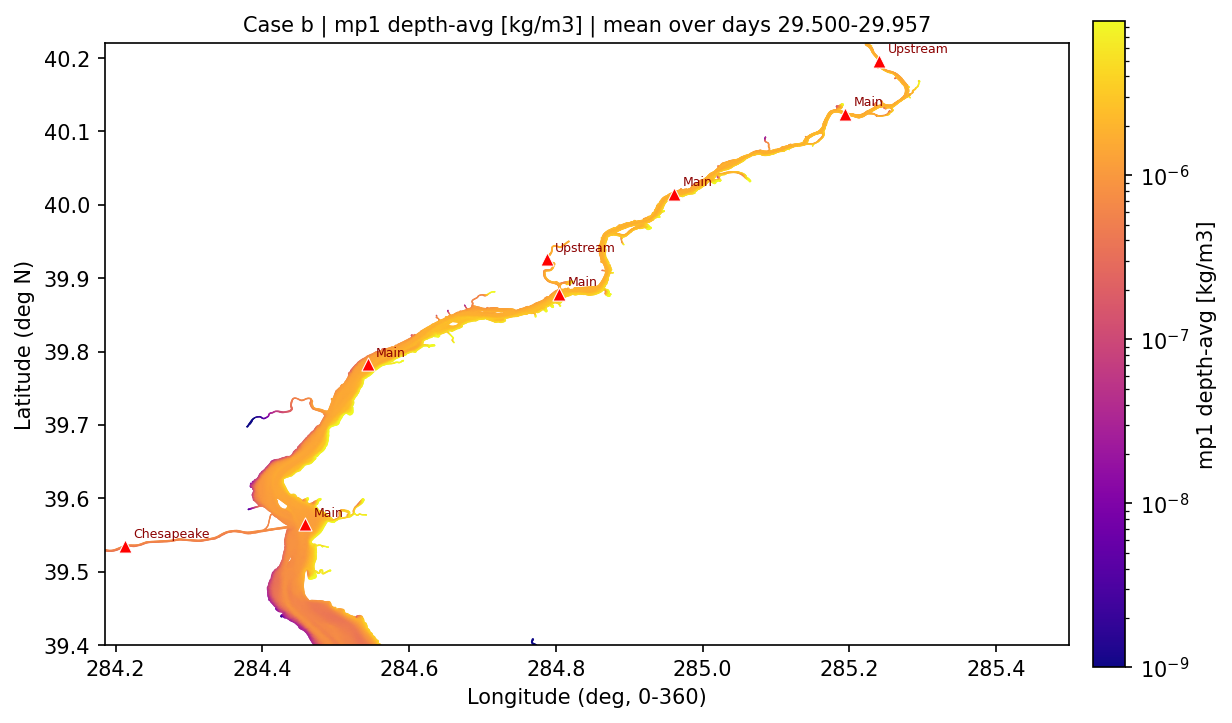
\includegraphics[width=\textwidth]{../FVCOM_MP_test_run/PYTHON/output/spatial_distribution/day30/planview_dayavg_mp1_davg_caseb.png}
  \caption{Case b}
\end{subfigure}
\hfill
\begin{subfigure}[b]{0.32\textwidth}
  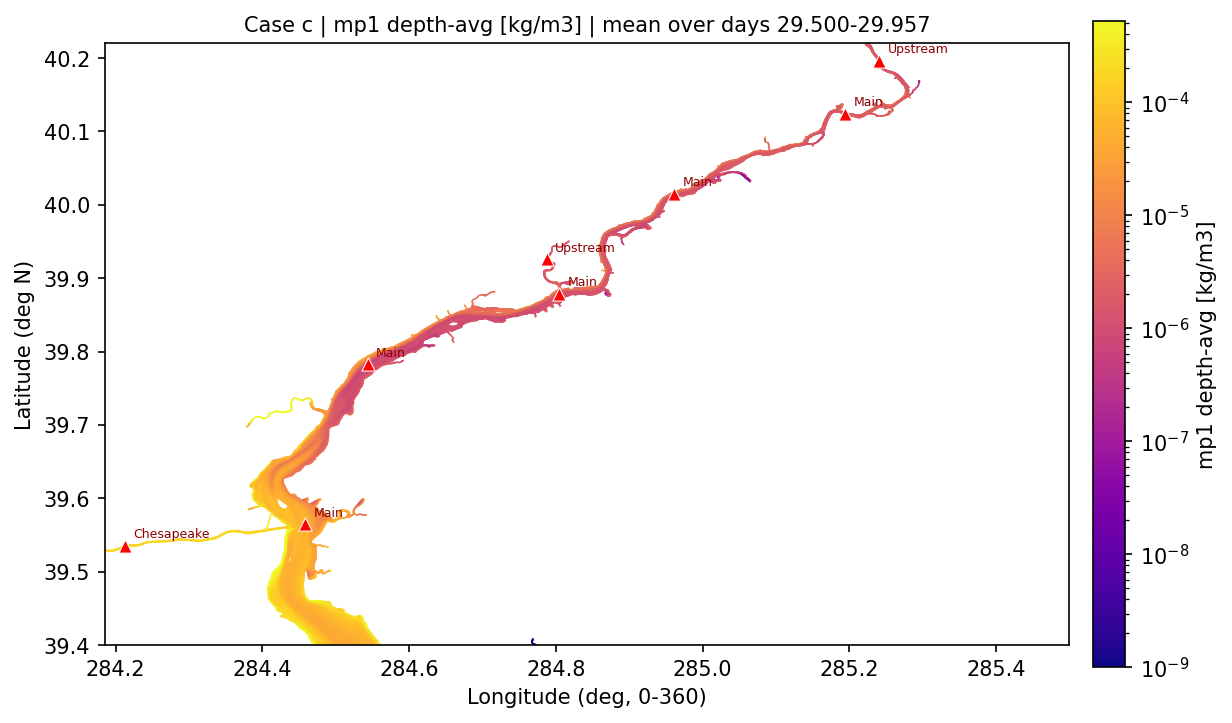
\includegraphics[width=\textwidth]{../FVCOM_MP_test_run/PYTHON/output/spatial_distribution/day30/planview_dayavg_mp1_davg_casec.png}
  \caption{Case c}
\end{subfigure}
\caption{Day-mean depth-averaged \texttt{mp1} concentration,
         simulation days 29.500--29.957.}
\label{fig:day30_mp1_davg}
\end{figure}

\subsection*{R2. Day-Mean Depth-Averaged mp1: Day 90}

\begin{figure}[H]
\centering
\begin{subfigure}[b]{0.32\textwidth}
  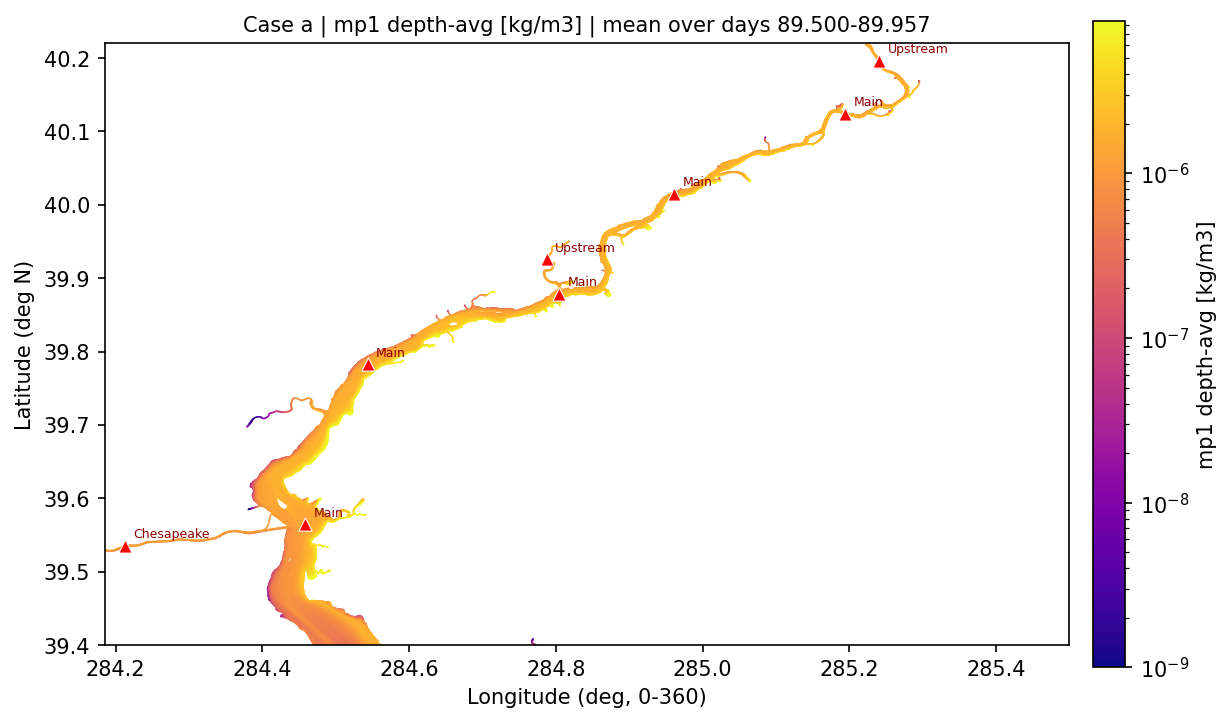
\includegraphics[width=\textwidth]{../FVCOM_MP_test_run/PYTHON/output/spatial_distribution/day90/planview_dayavg_mp1_davg_casea.png}
  \caption{Case a}
\end{subfigure}
\hfill
\begin{subfigure}[b]{0.32\textwidth}
  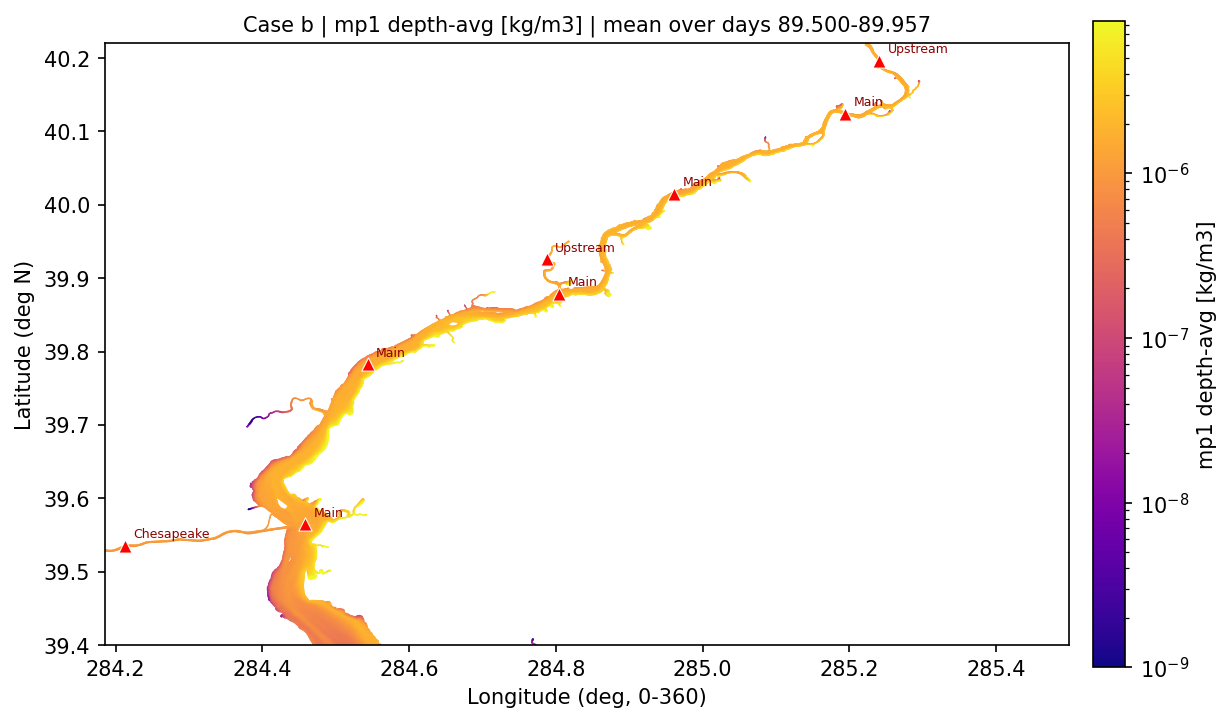
\includegraphics[width=\textwidth]{../FVCOM_MP_test_run/PYTHON/output/spatial_distribution/day90/planview_dayavg_mp1_davg_caseb.png}
  \caption{Case b}
\end{subfigure}
\hfill
\begin{subfigure}[b]{0.32\textwidth}
  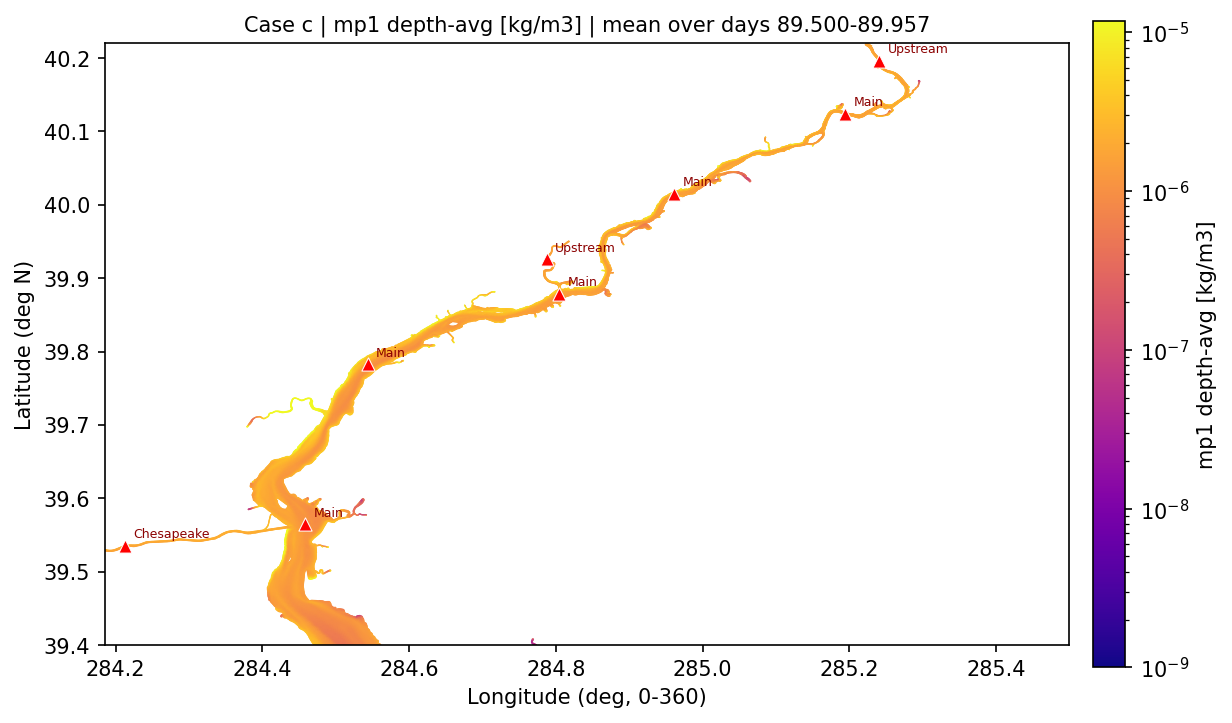
\includegraphics[width=\textwidth]{../FVCOM_MP_test_run/PYTHON/output/spatial_distribution/day90/planview_dayavg_mp1_davg_casec.png}
  \caption{Case c}
\end{subfigure}
\caption{Day-mean depth-averaged \texttt{mp1} concentration,
         simulation days 89.500--89.957.}
\label{fig:day90_mp1_davg}
\end{figure}

\subsection*{R3. Floc-Component Split in Case c}

\begin{figure}[H]
\centering
\begin{subfigure}[b]{0.24\textwidth}
  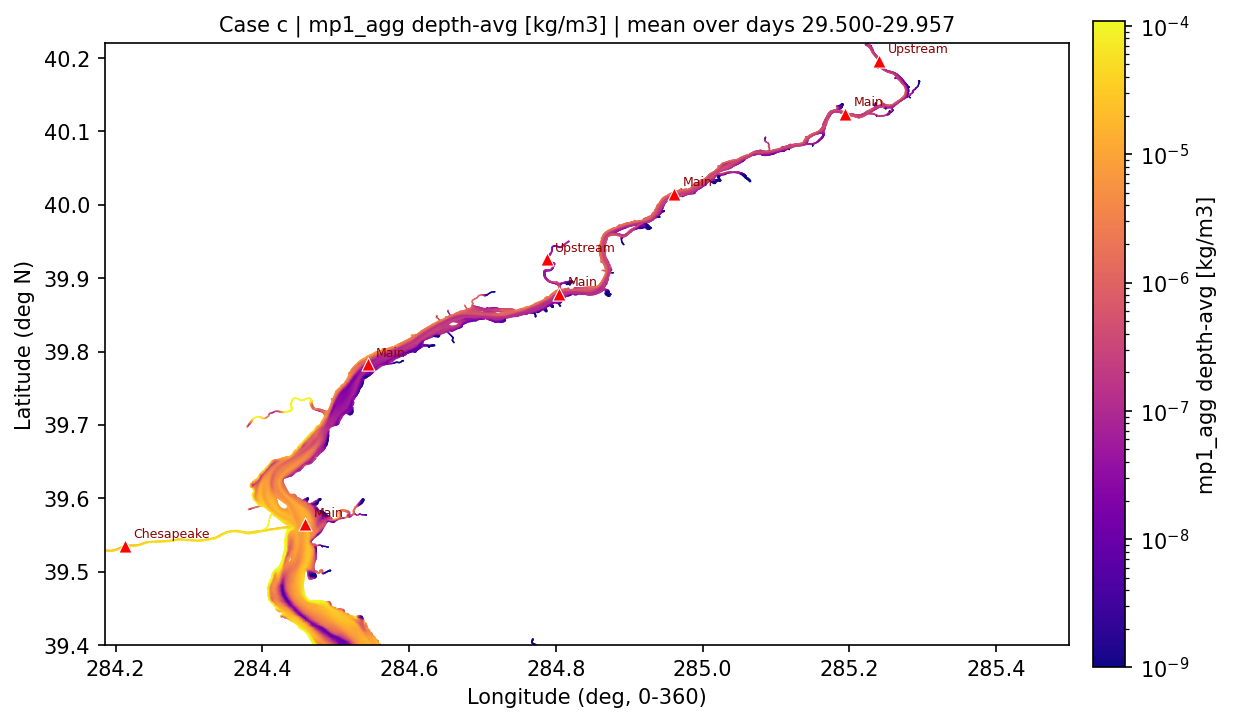
\includegraphics[width=\textwidth]{../FVCOM_MP_test_run/PYTHON/output/spatial_distribution/day30/planview_dayavg_mp1_agg_davg_casec.png}
  \caption{Day 30 agg}
\end{subfigure}
\hfill
\begin{subfigure}[b]{0.24\textwidth}
  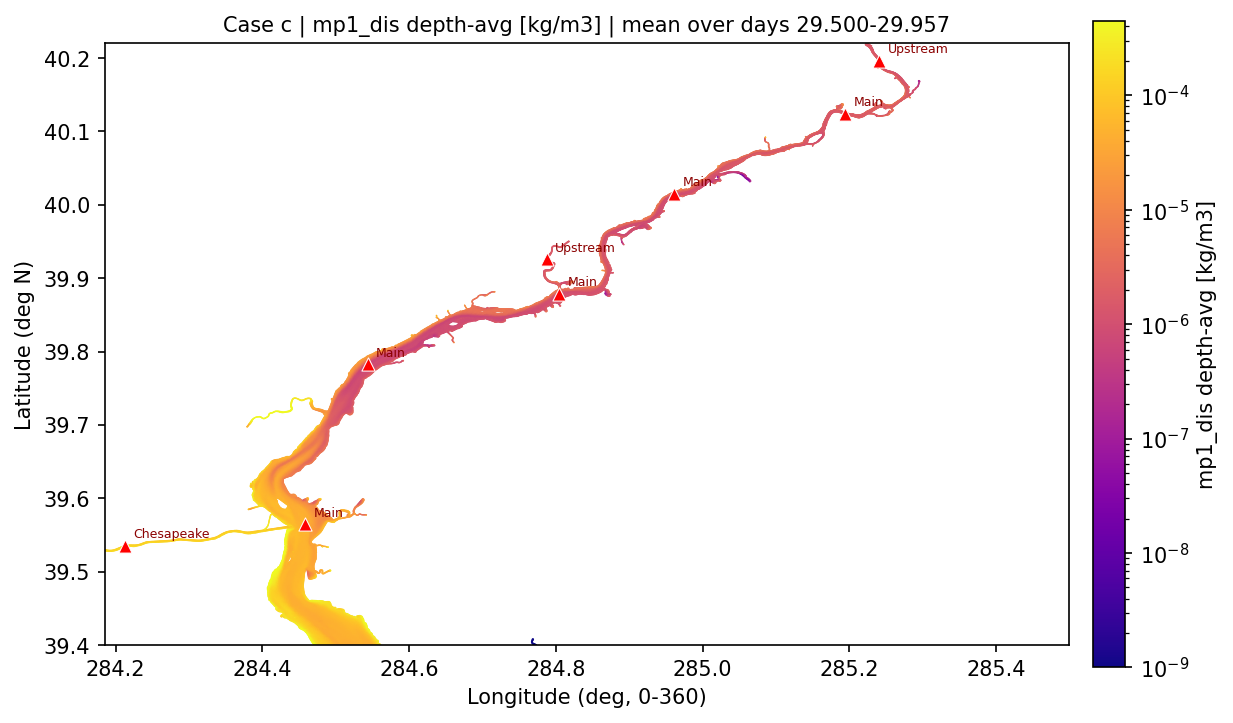
\includegraphics[width=\textwidth]{../FVCOM_MP_test_run/PYTHON/output/spatial_distribution/day30/planview_dayavg_mp1_dis_davg_casec.png}
  \caption{Day 30 dis}
\end{subfigure}
\hfill
\begin{subfigure}[b]{0.24\textwidth}
  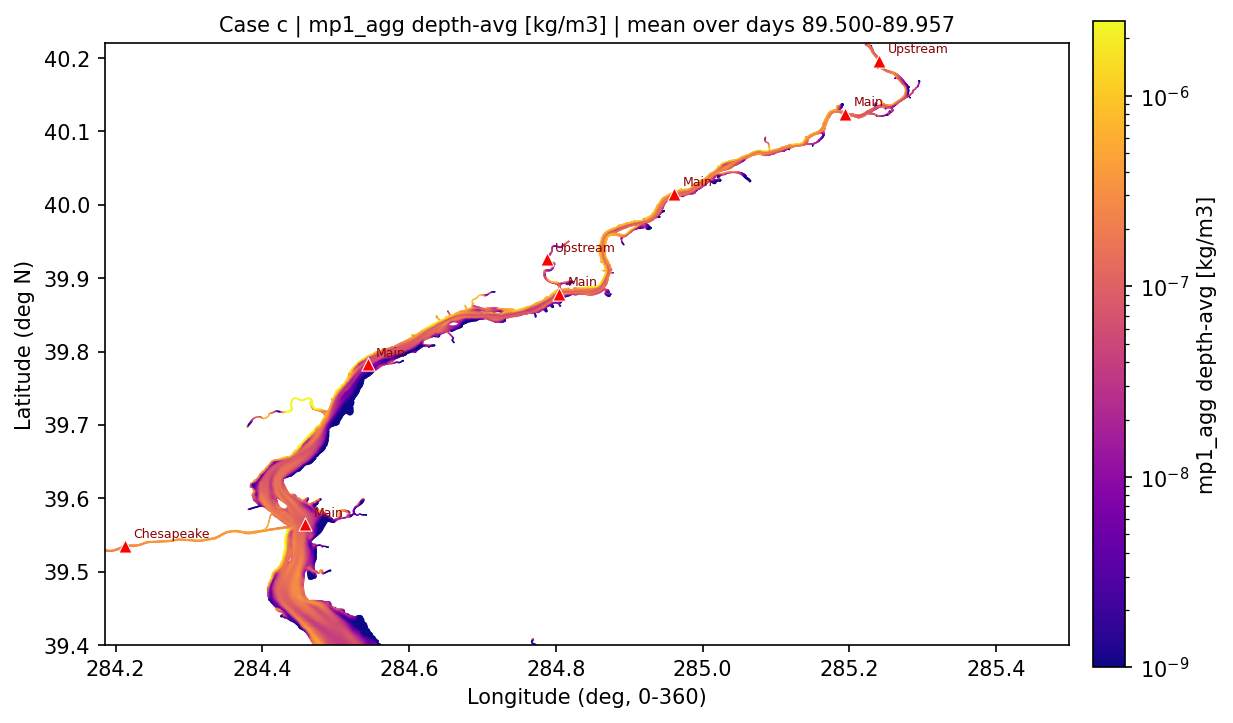
\includegraphics[width=\textwidth]{../FVCOM_MP_test_run/PYTHON/output/spatial_distribution/day90/planview_dayavg_mp1_agg_davg_casec.png}
  \caption{Day 90 agg}
\end{subfigure}
\hfill
\begin{subfigure}[b]{0.24\textwidth}
  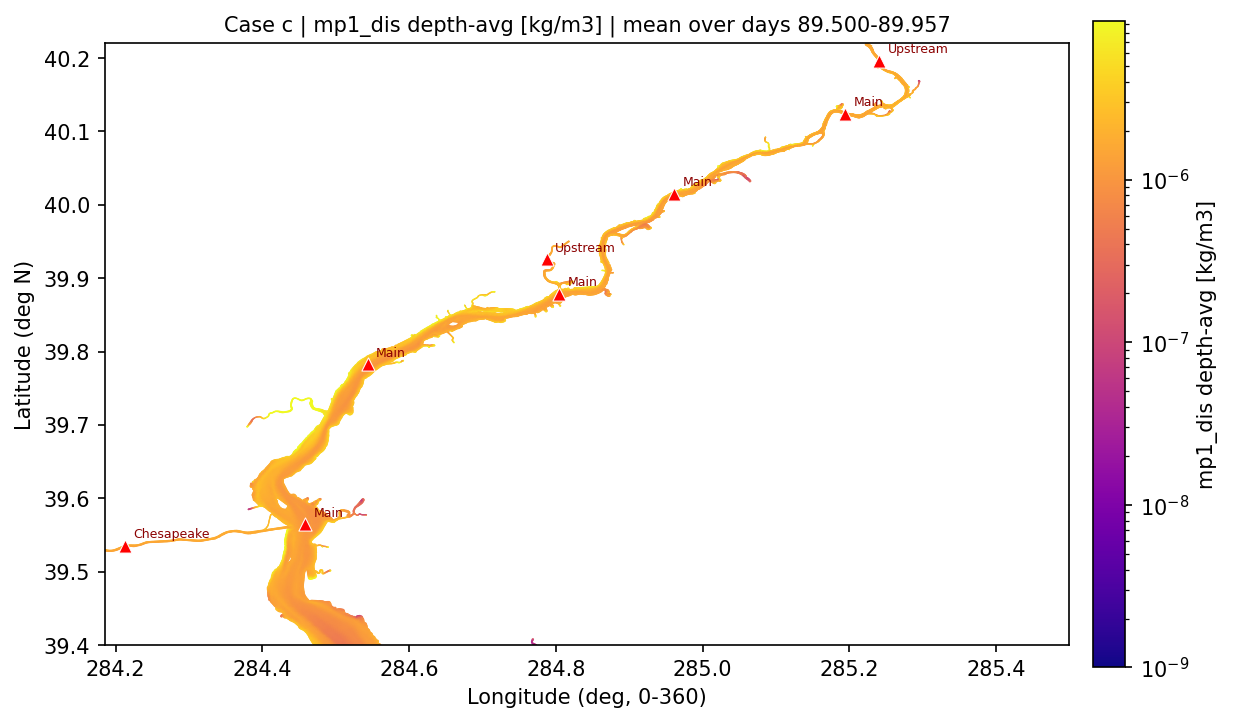
\includegraphics[width=\textwidth]{../FVCOM_MP_test_run/PYTHON/output/spatial_distribution/day90/planview_dayavg_mp1_dis_davg_casec.png}
  \caption{Day 90 dis}
\end{subfigure}
\caption{Depth-averaged aggregated and disaggregated plastic components in
         case~\texttt{c}.  Case~\texttt{b} has zero aggregated component in
         both late-time windows.}
\label{fig:casec_split}
\end{figure}

\subsection*{R4. Bed Plastic Mass Density}

\begin{figure}[H]
\centering
\begin{subfigure}[b]{0.32\textwidth}
  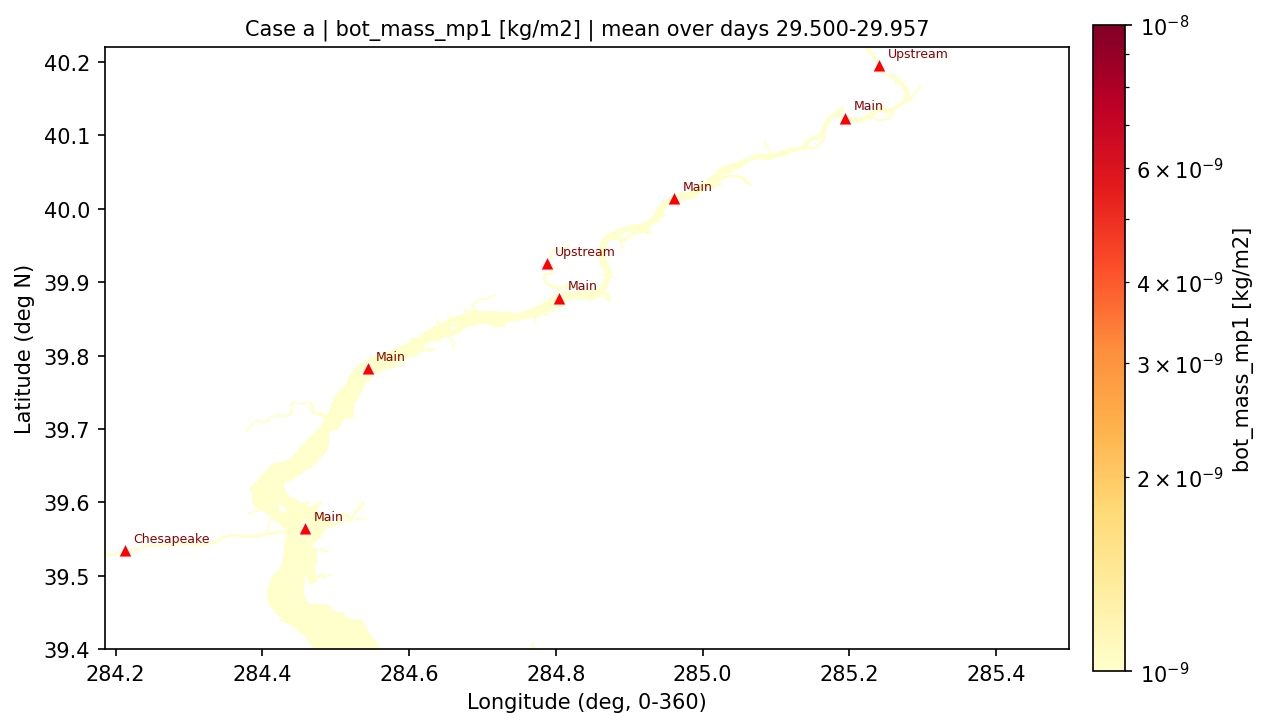
\includegraphics[width=\textwidth]{../FVCOM_MP_test_run/PYTHON/output/spatial_distribution/day30/planview_dayavg_bot_mass_casea.png}
  \caption{Day 30 case a}
\end{subfigure}
\hfill
\begin{subfigure}[b]{0.32\textwidth}
  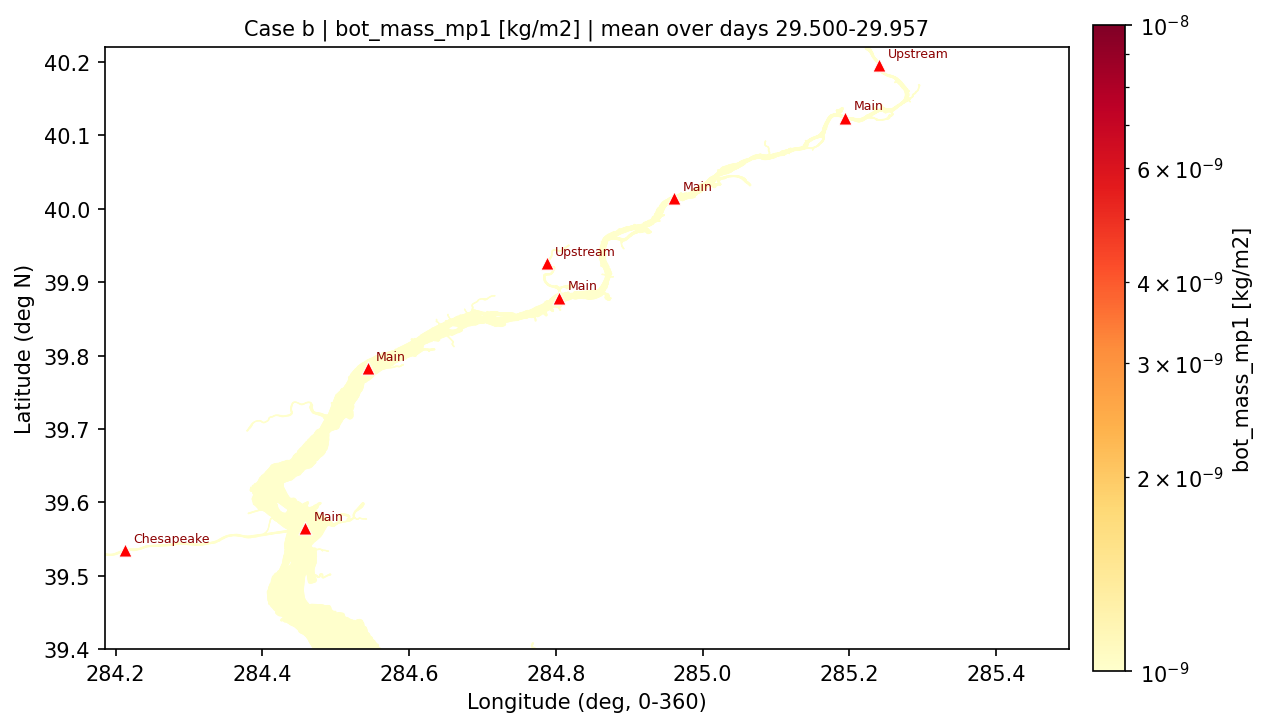
\includegraphics[width=\textwidth]{../FVCOM_MP_test_run/PYTHON/output/spatial_distribution/day30/planview_dayavg_bot_mass_caseb.png}
  \caption{Day 30 case b}
\end{subfigure}
\hfill
\begin{subfigure}[b]{0.32\textwidth}
  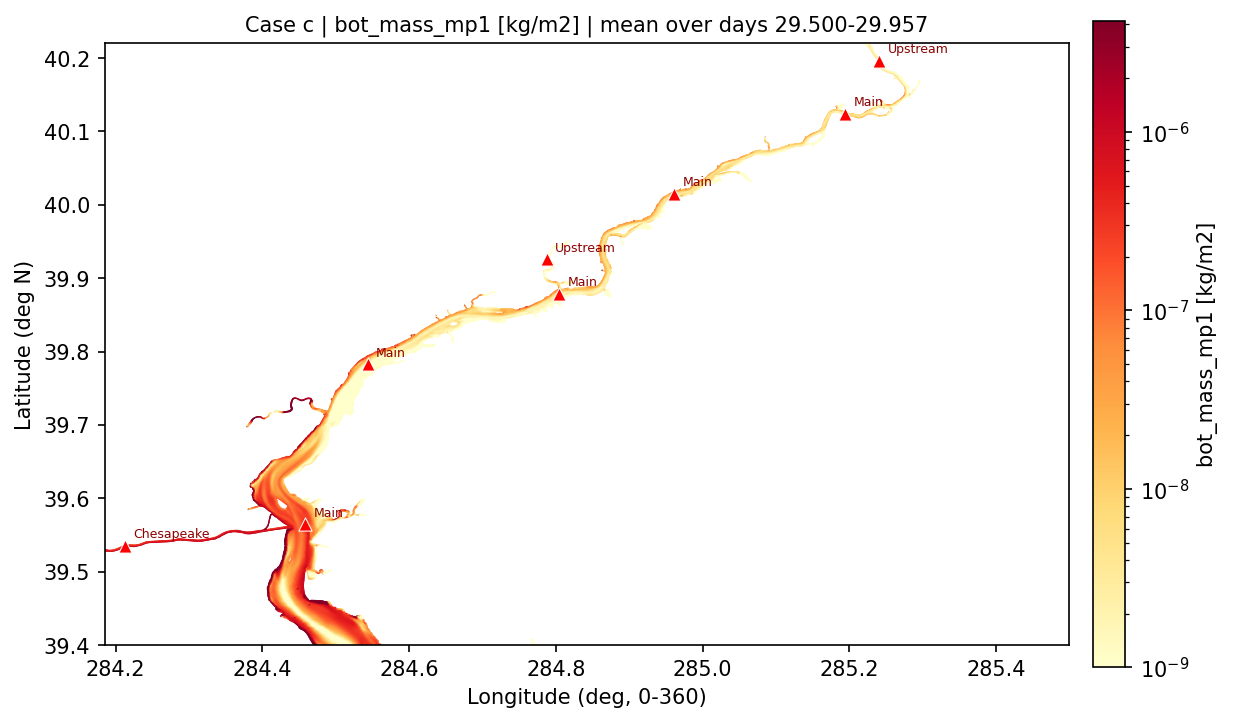
\includegraphics[width=\textwidth]{../FVCOM_MP_test_run/PYTHON/output/spatial_distribution/day30/planview_dayavg_bot_mass_casec.png}
  \caption{Day 30 case c}
\end{subfigure}

\vspace{0.8em}

\begin{subfigure}[b]{0.32\textwidth}
  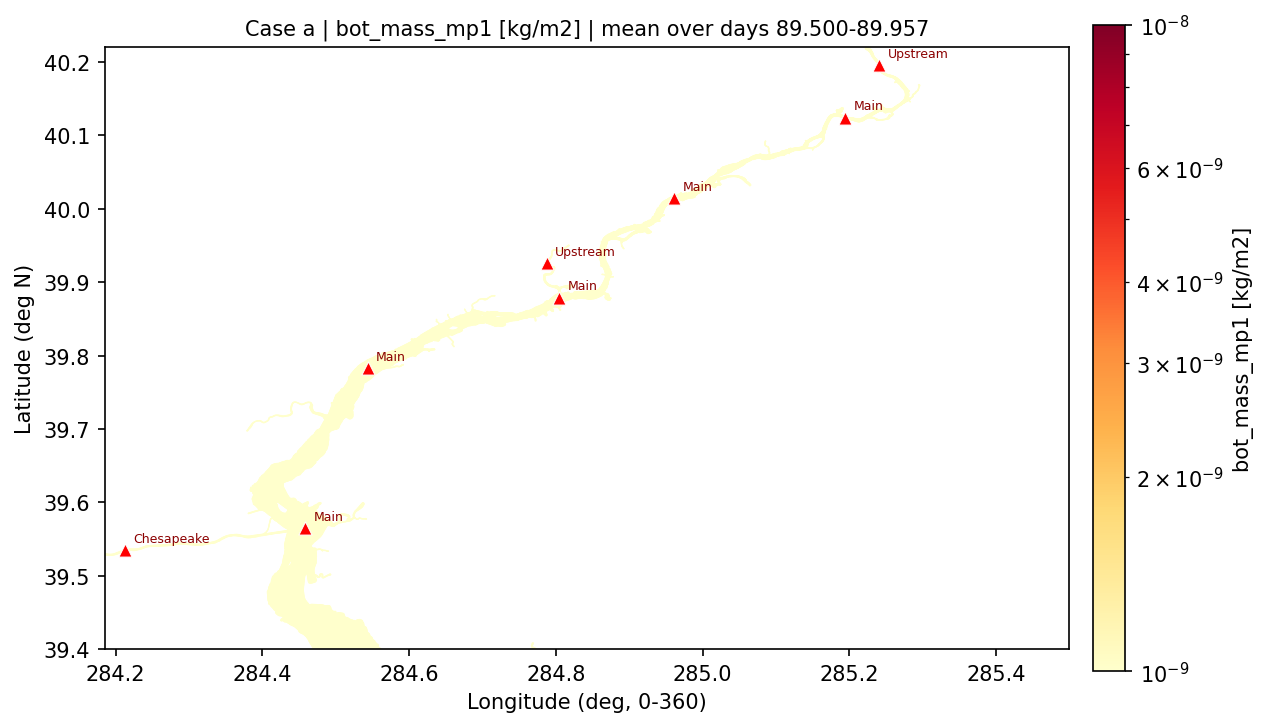
\includegraphics[width=\textwidth]{../FVCOM_MP_test_run/PYTHON/output/spatial_distribution/day90/planview_dayavg_bot_mass_casea.png}
  \caption{Day 90 case a}
\end{subfigure}
\hfill
\begin{subfigure}[b]{0.32\textwidth}
  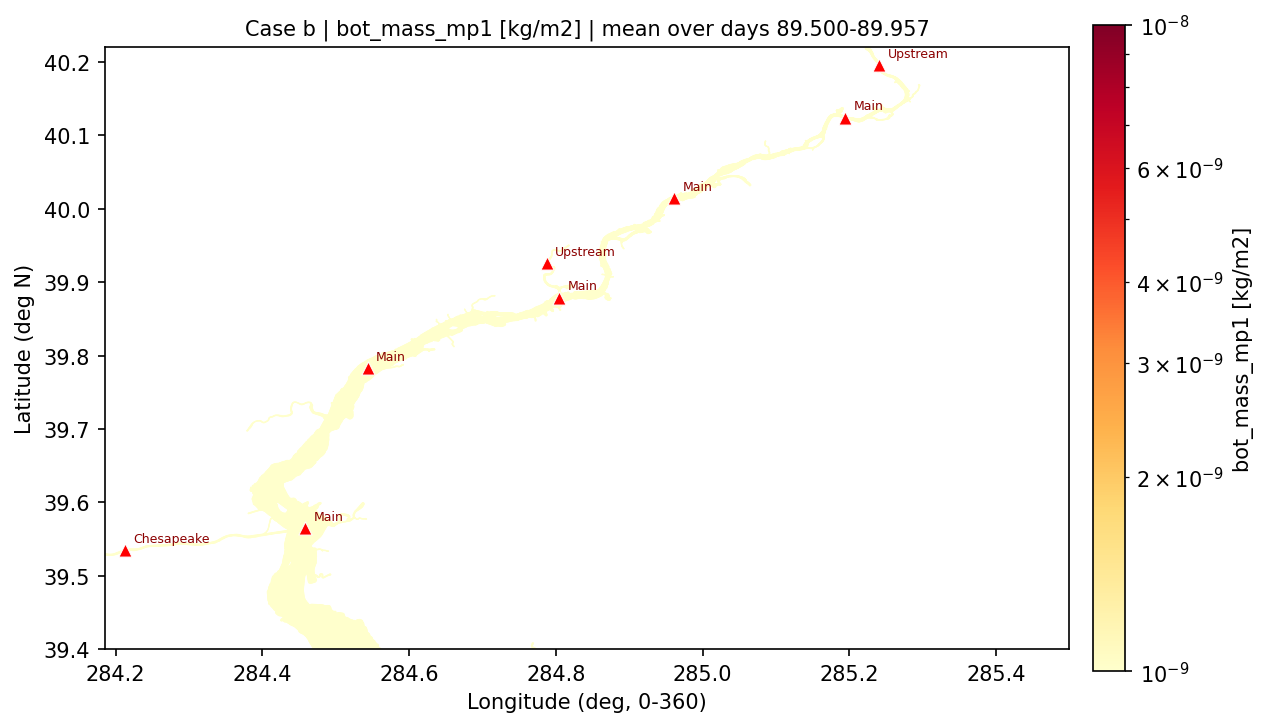
\includegraphics[width=\textwidth]{../FVCOM_MP_test_run/PYTHON/output/spatial_distribution/day90/planview_dayavg_bot_mass_caseb.png}
  \caption{Day 90 case b}
\end{subfigure}
\hfill
\begin{subfigure}[b]{0.32\textwidth}
  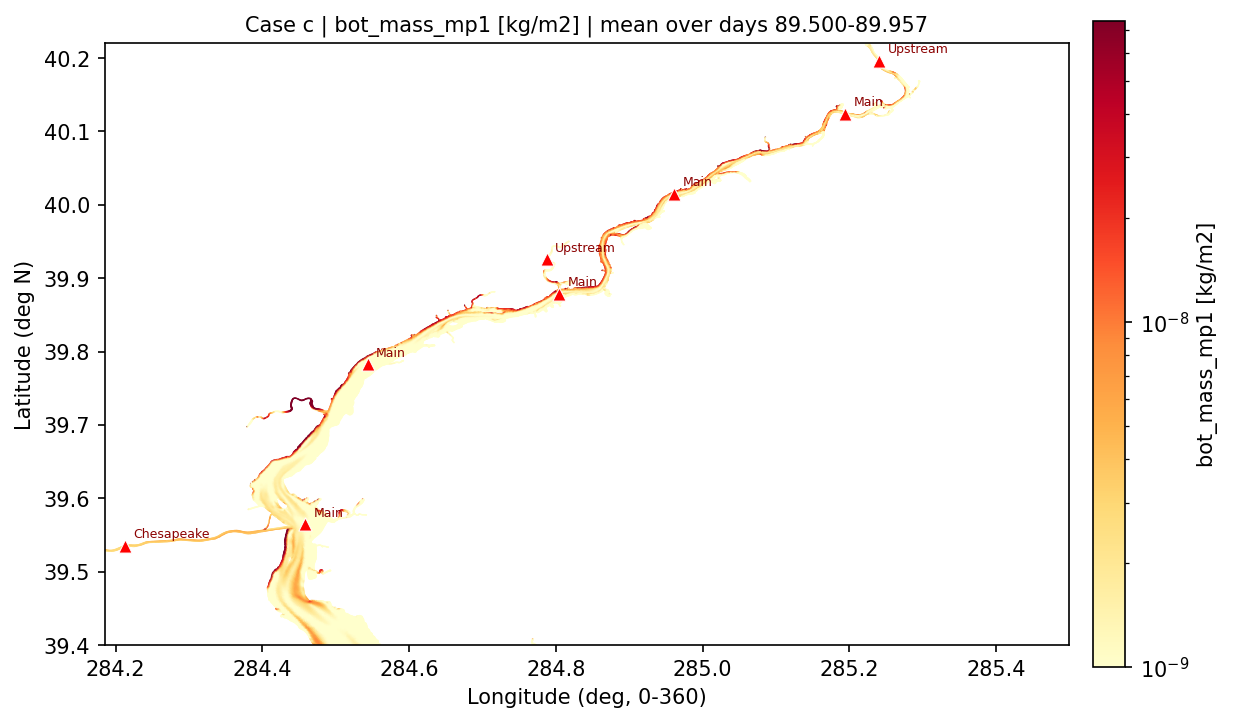
\includegraphics[width=\textwidth]{../FVCOM_MP_test_run/PYTHON/output/spatial_distribution/day90/planview_dayavg_bot_mass_casec.png}
  \caption{Day 90 case c}
\end{subfigure}
\caption{Day-mean bed plastic mass density for late-time windows.  Cases
         \texttt{a} and \texttt{b} remain zero; case~\texttt{c} retains
         active bed mass, with a lower point maximum in the day~90 window
         than in the day~30 window.}
\label{fig:bot_mass_late}
\end{figure}

\subsection*{R5. Pointwise-Maximum Depth-Averaged mp1}

\begin{figure}[H]
\centering
\begin{subfigure}[b]{0.32\textwidth}
  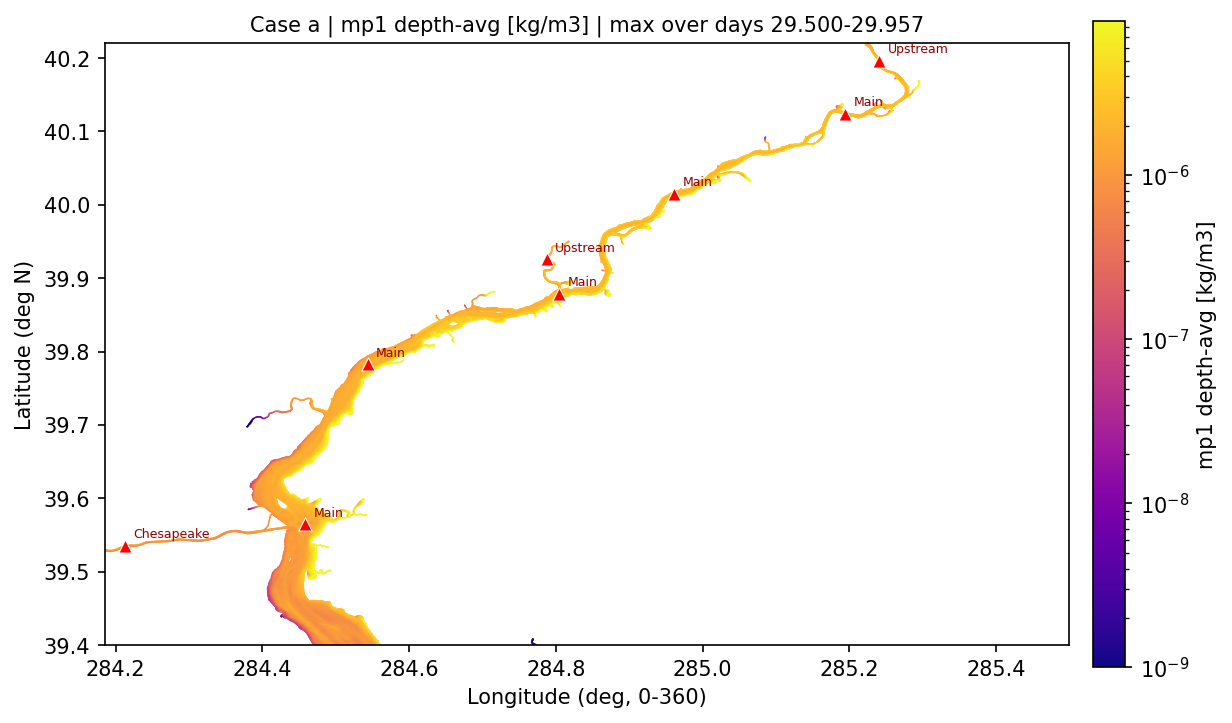
\includegraphics[width=\textwidth]{../FVCOM_MP_test_run/PYTHON/output/spatial_distribution/day30/planview_max_mp1_davg_casea.png}
  \caption{Day 30 case a}
\end{subfigure}
\hfill
\begin{subfigure}[b]{0.32\textwidth}
  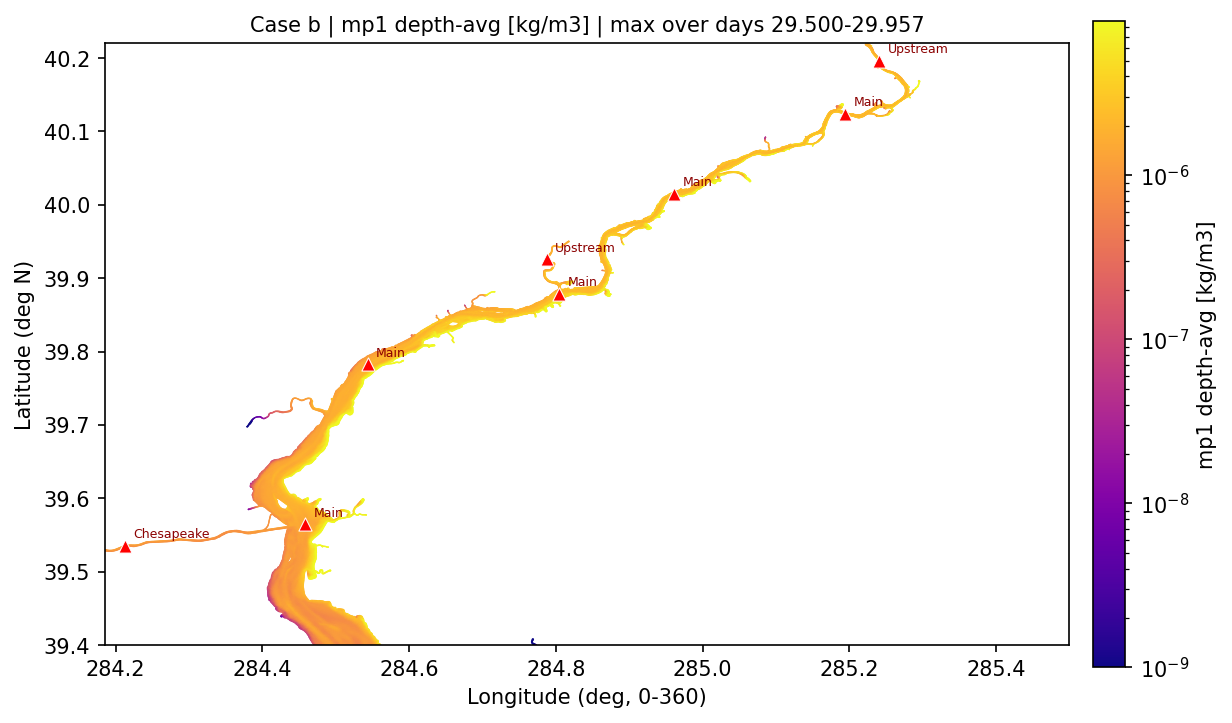
\includegraphics[width=\textwidth]{../FVCOM_MP_test_run/PYTHON/output/spatial_distribution/day30/planview_max_mp1_davg_caseb.png}
  \caption{Day 30 case b}
\end{subfigure}
\hfill
\begin{subfigure}[b]{0.32\textwidth}
  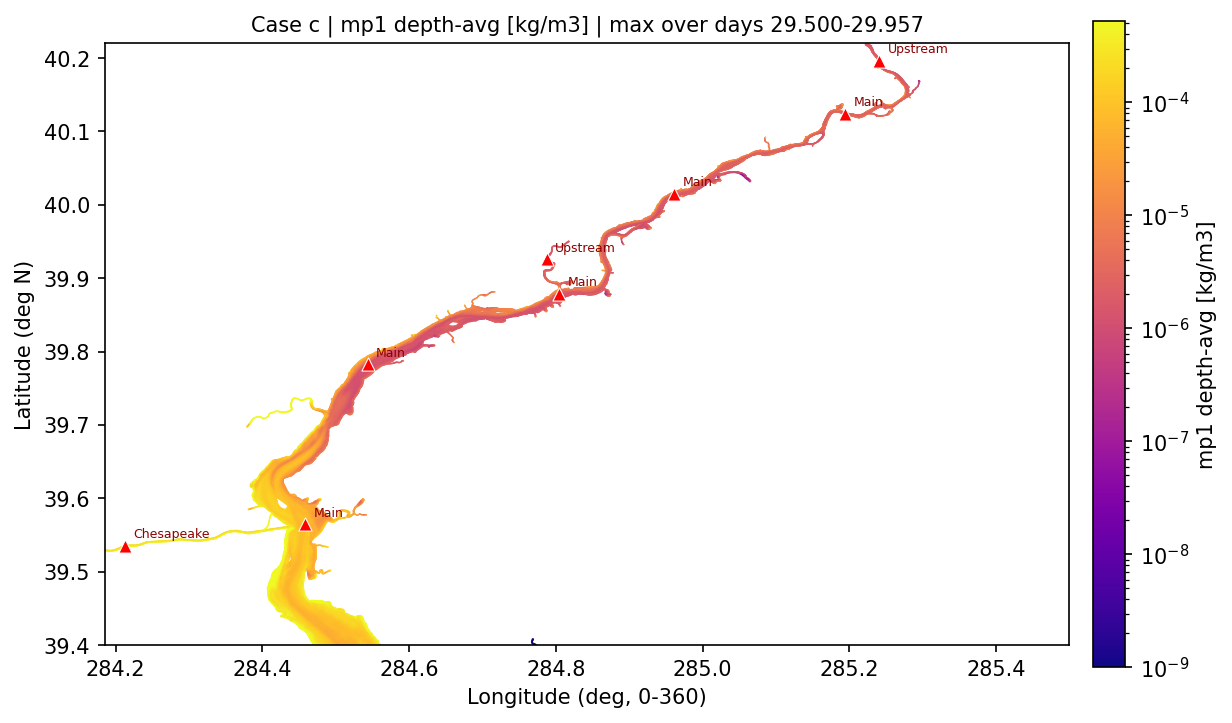
\includegraphics[width=\textwidth]{../FVCOM_MP_test_run/PYTHON/output/spatial_distribution/day30/planview_max_mp1_davg_casec.png}
  \caption{Day 30 case c}
\end{subfigure}

\vspace{0.8em}

\begin{subfigure}[b]{0.32\textwidth}
  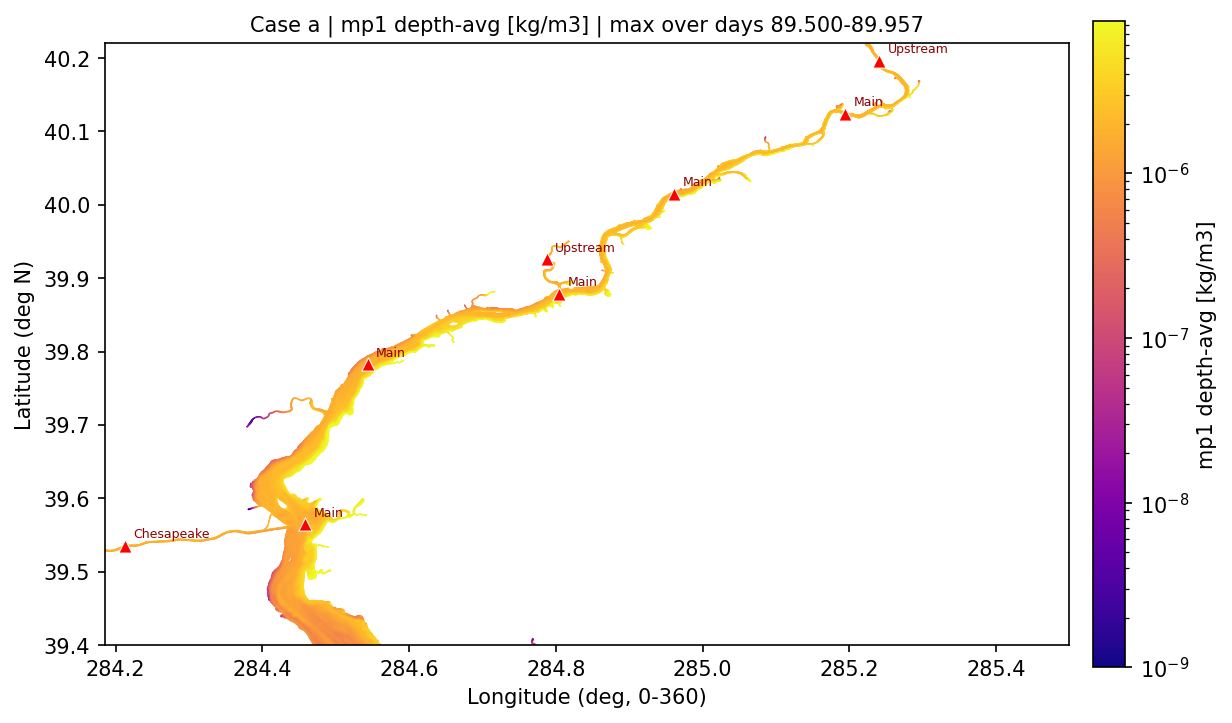
\includegraphics[width=\textwidth]{../FVCOM_MP_test_run/PYTHON/output/spatial_distribution/day90/planview_max_mp1_davg_casea.png}
  \caption{Day 90 case a}
\end{subfigure}
\hfill
\begin{subfigure}[b]{0.32\textwidth}
  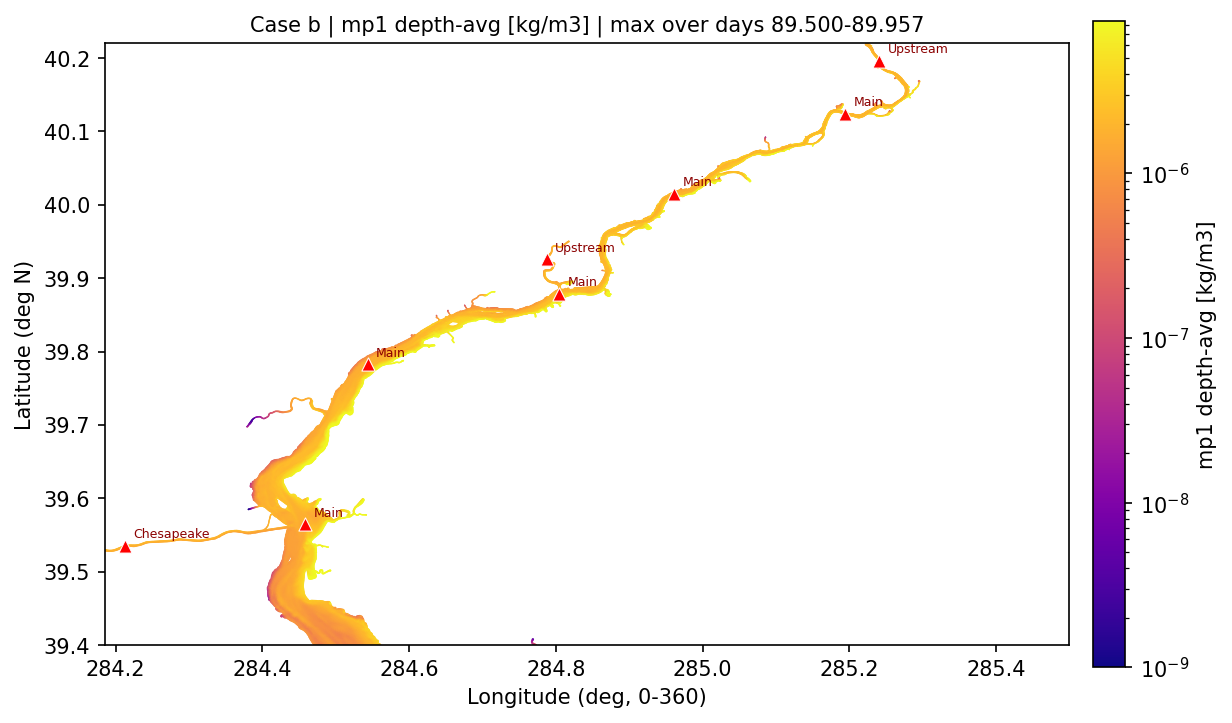
\includegraphics[width=\textwidth]{../FVCOM_MP_test_run/PYTHON/output/spatial_distribution/day90/planview_max_mp1_davg_caseb.png}
  \caption{Day 90 case b}
\end{subfigure}
\hfill
\begin{subfigure}[b]{0.32\textwidth}
  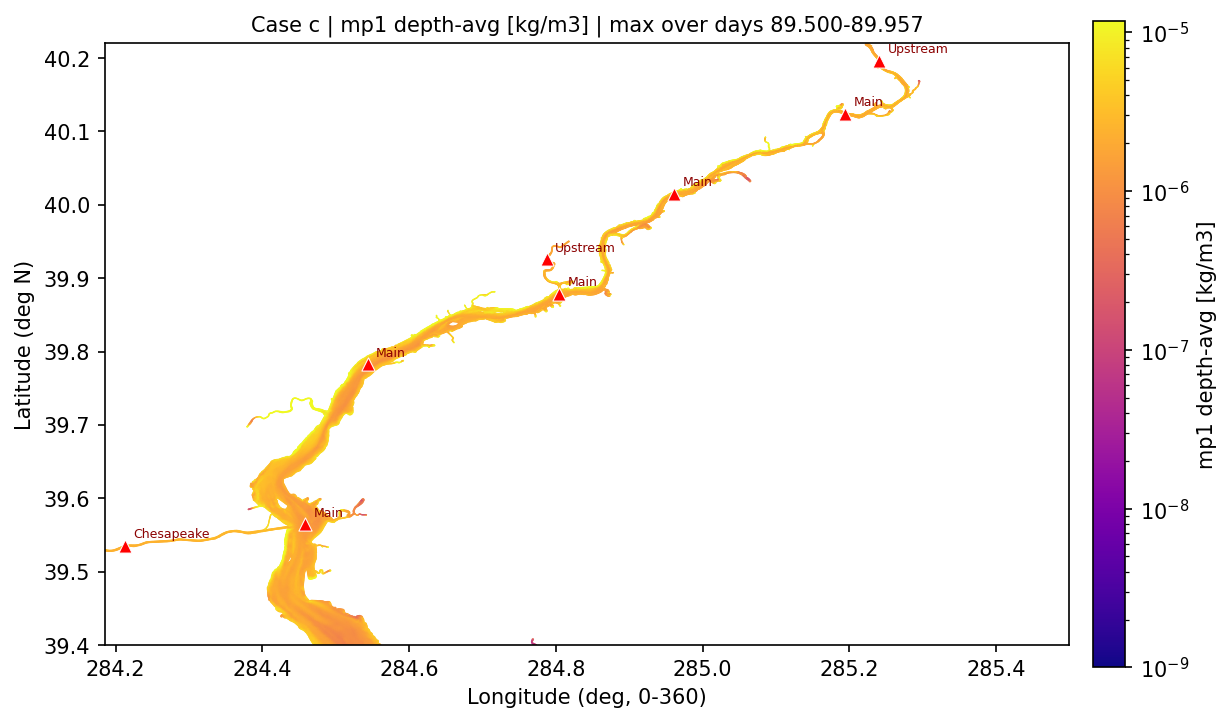
\includegraphics[width=\textwidth]{../FVCOM_MP_test_run/PYTHON/output/spatial_distribution/day90/planview_max_mp1_davg_casec.png}
  \caption{Day 90 case c}
\end{subfigure}
\caption{Pointwise maximum depth-averaged \texttt{mp1} over each selected
         late-time window.  The maxima remain connected to the river/bay
         plume structure rather than appearing as detached single-node
         artifacts.}
\label{fig:max_mp1_late}
\end{figure}

\subsection*{R6. Cross-Case Difference Maps}

\begin{figure}[H]
\centering
\begin{subfigure}[b]{0.32\textwidth}
  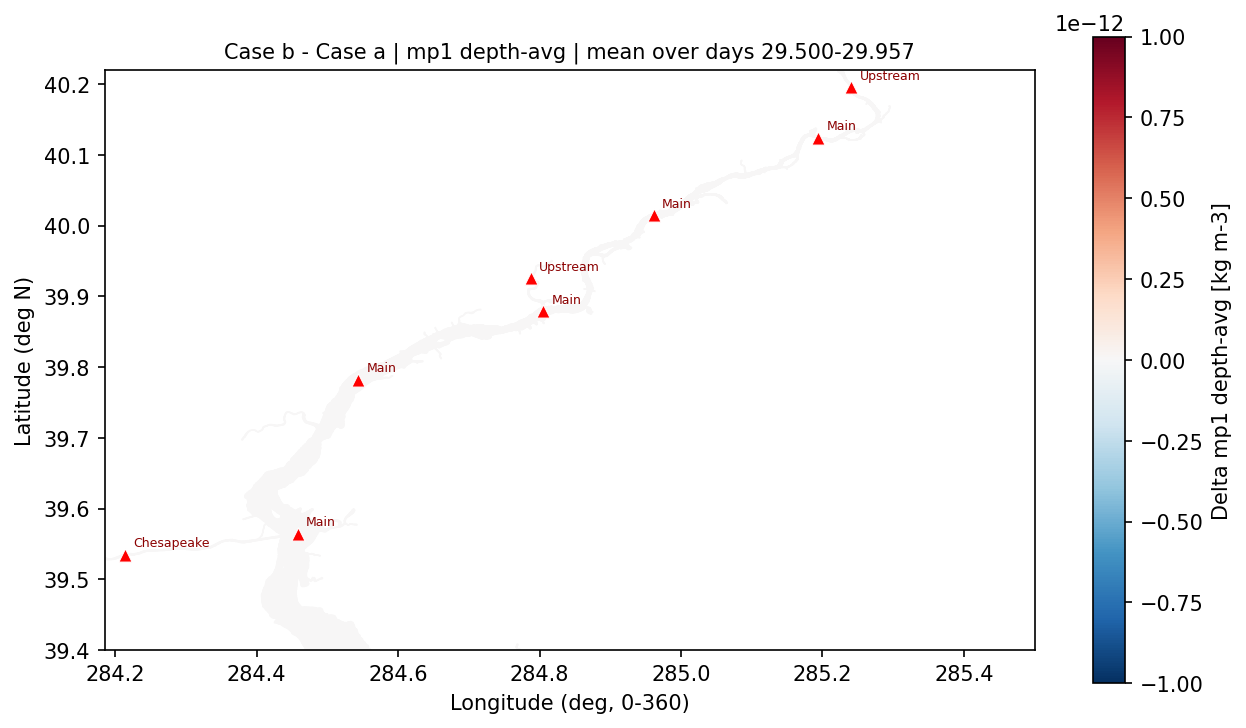
\includegraphics[width=\textwidth]{../FVCOM_MP_test_run/PYTHON/output/spatial_distribution/day30/diff_mp1_davg_caseb_minus_casea.png}
  \caption{Day 30 b-a}
\end{subfigure}
\hfill
\begin{subfigure}[b]{0.32\textwidth}
  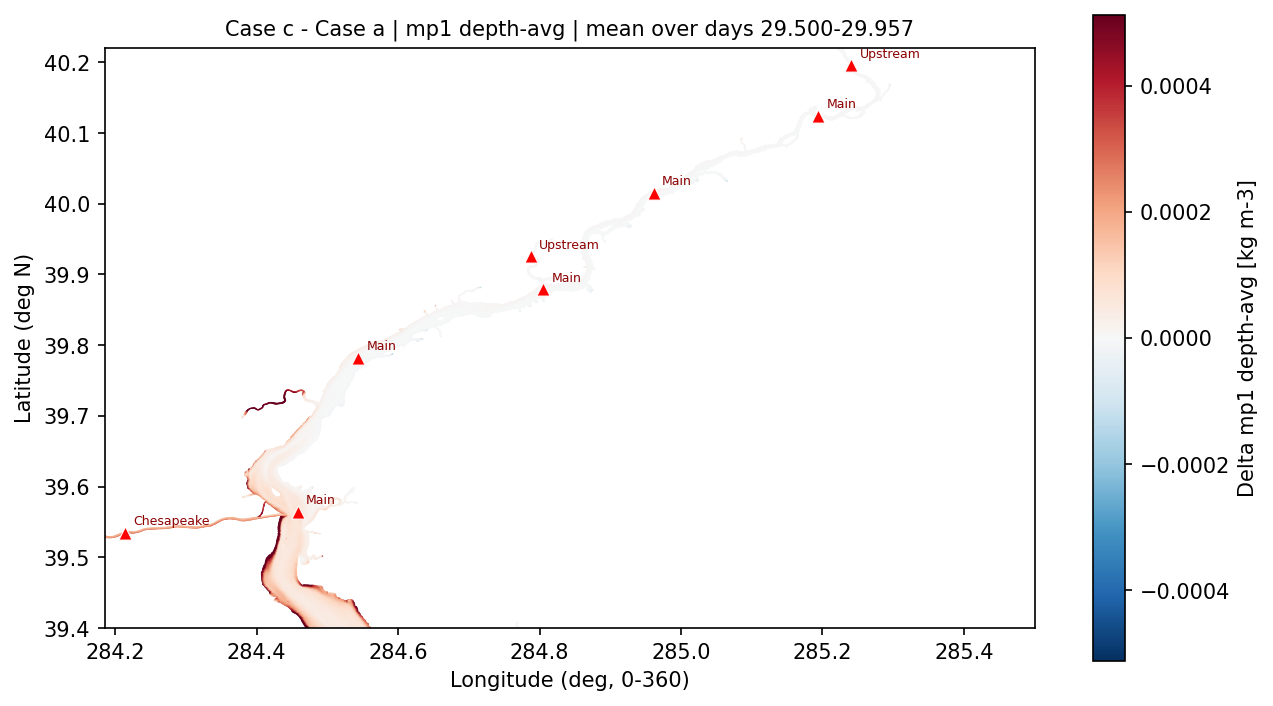
\includegraphics[width=\textwidth]{../FVCOM_MP_test_run/PYTHON/output/spatial_distribution/day30/diff_mp1_davg_casec_minus_casea.png}
  \caption{Day 30 c-a}
\end{subfigure}
\hfill
\begin{subfigure}[b]{0.32\textwidth}
  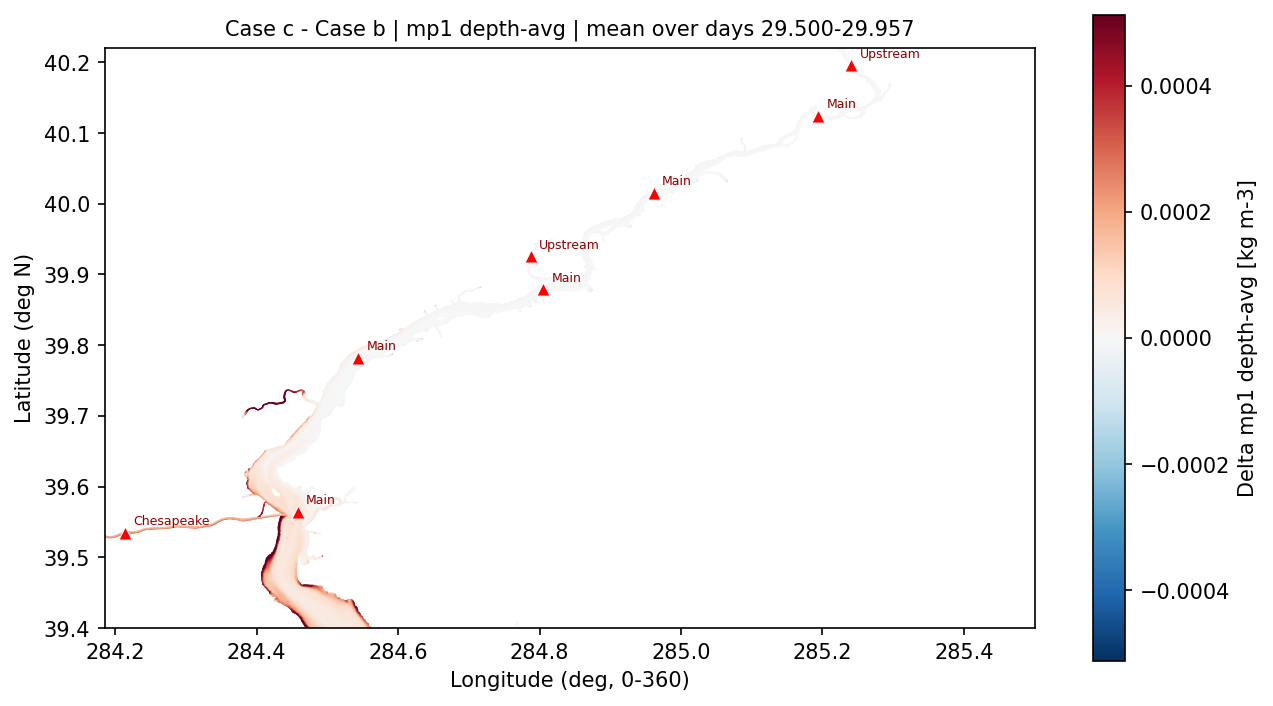
\includegraphics[width=\textwidth]{../FVCOM_MP_test_run/PYTHON/output/spatial_distribution/day30/diff_mp1_davg_casec_minus_caseb.png}
  \caption{Day 30 c-b}
\end{subfigure}

\vspace{0.8em}

\begin{subfigure}[b]{0.32\textwidth}
  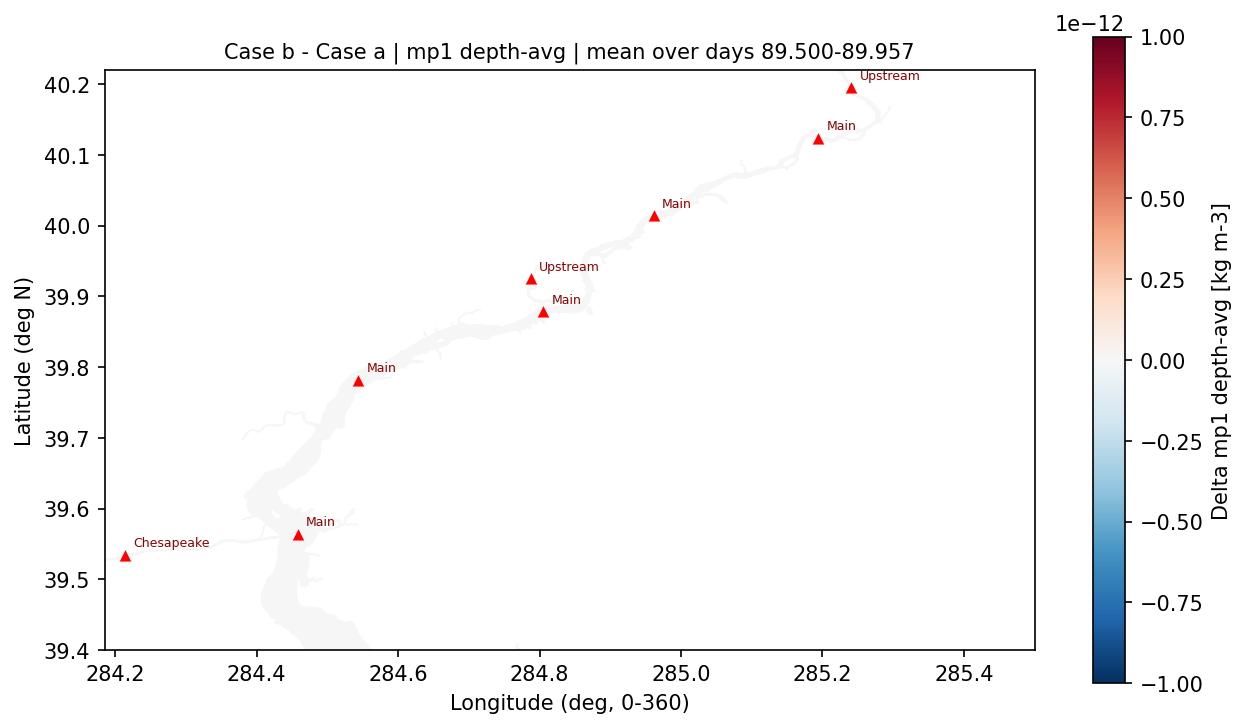
\includegraphics[width=\textwidth]{../FVCOM_MP_test_run/PYTHON/output/spatial_distribution/day90/diff_mp1_davg_caseb_minus_casea.png}
  \caption{Day 90 b-a}
\end{subfigure}
\hfill
\begin{subfigure}[b]{0.32\textwidth}
  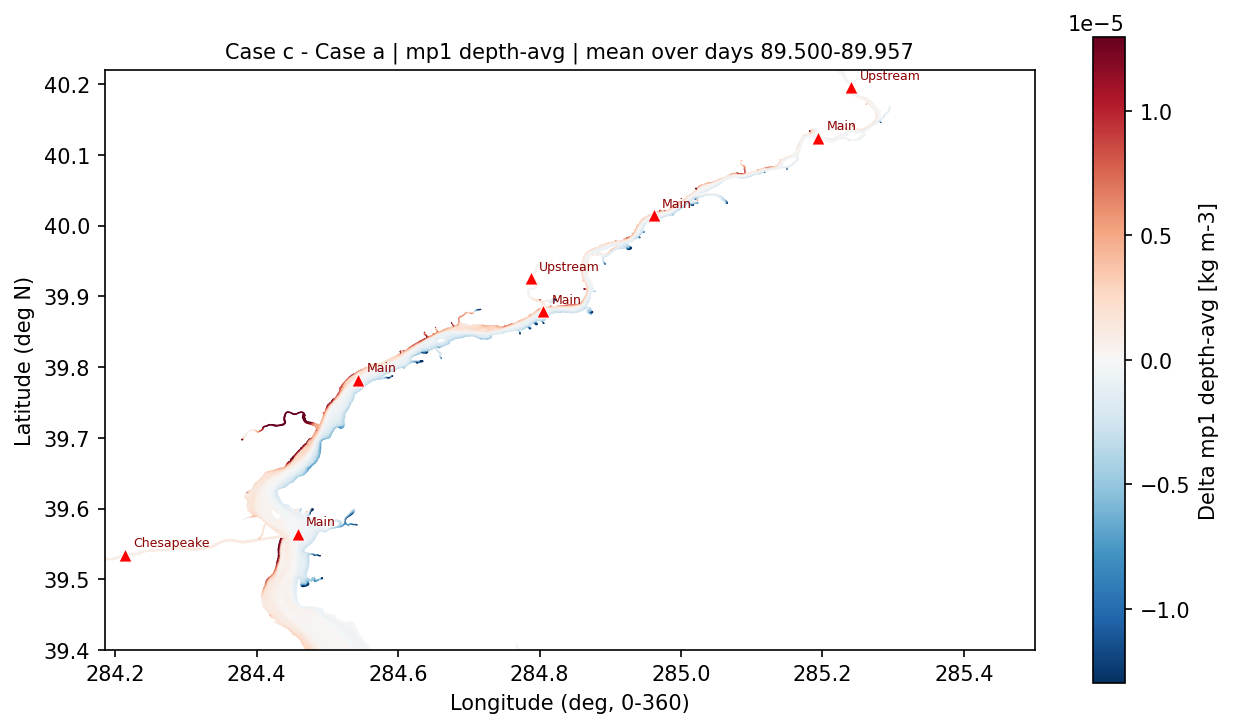
\includegraphics[width=\textwidth]{../FVCOM_MP_test_run/PYTHON/output/spatial_distribution/day90/diff_mp1_davg_casec_minus_casea.png}
  \caption{Day 90 c-a}
\end{subfigure}
\hfill
\begin{subfigure}[b]{0.32\textwidth}
  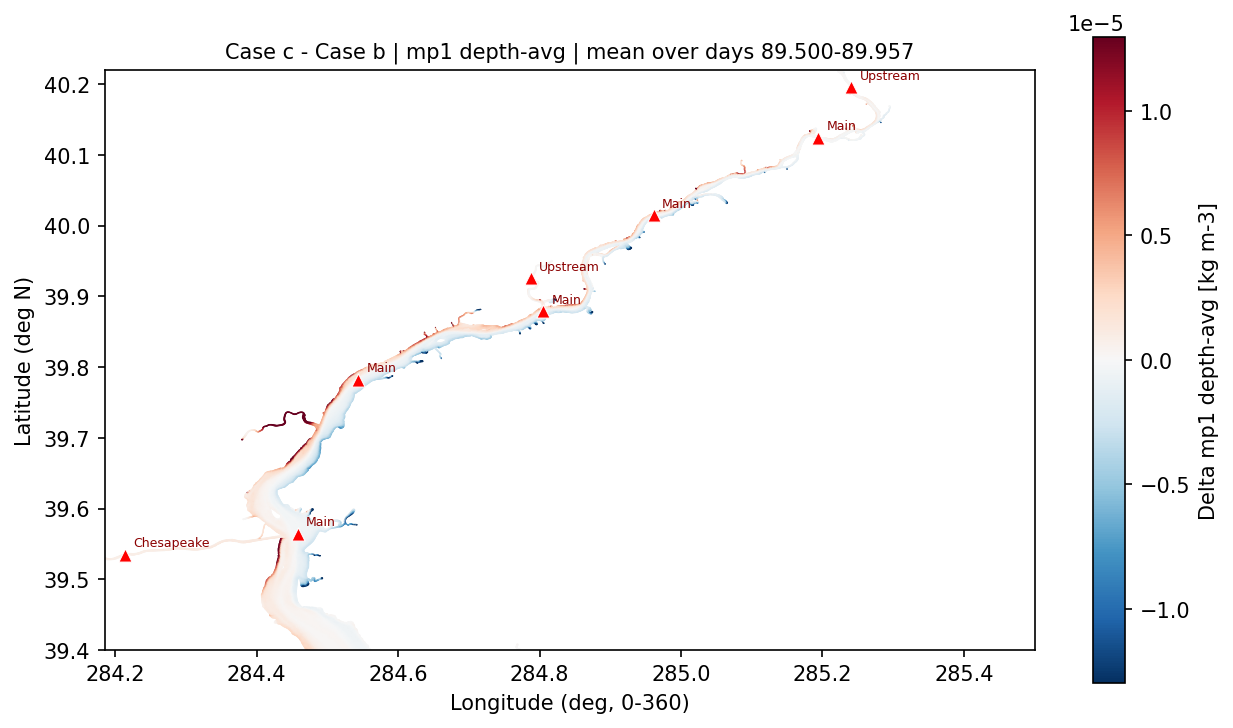
\includegraphics[width=\textwidth]{../FVCOM_MP_test_run/PYTHON/output/spatial_distribution/day90/diff_mp1_davg_casec_minus_caseb.png}
  \caption{Day 90 c-b}
\end{subfigure}
\caption{Day-mean cross-case differences for depth-averaged \texttt{mp1}.
         The b-a panels are zero in the CSV diagnostics; c-a and c-b isolate
         the floc-enabled redistribution in corrected case~\texttt{c}.}
\label{fig:diff_mp1_late}
\end{figure}

\subsection*{R7. Station Time Series}

\begin{figure}[H]
\centering
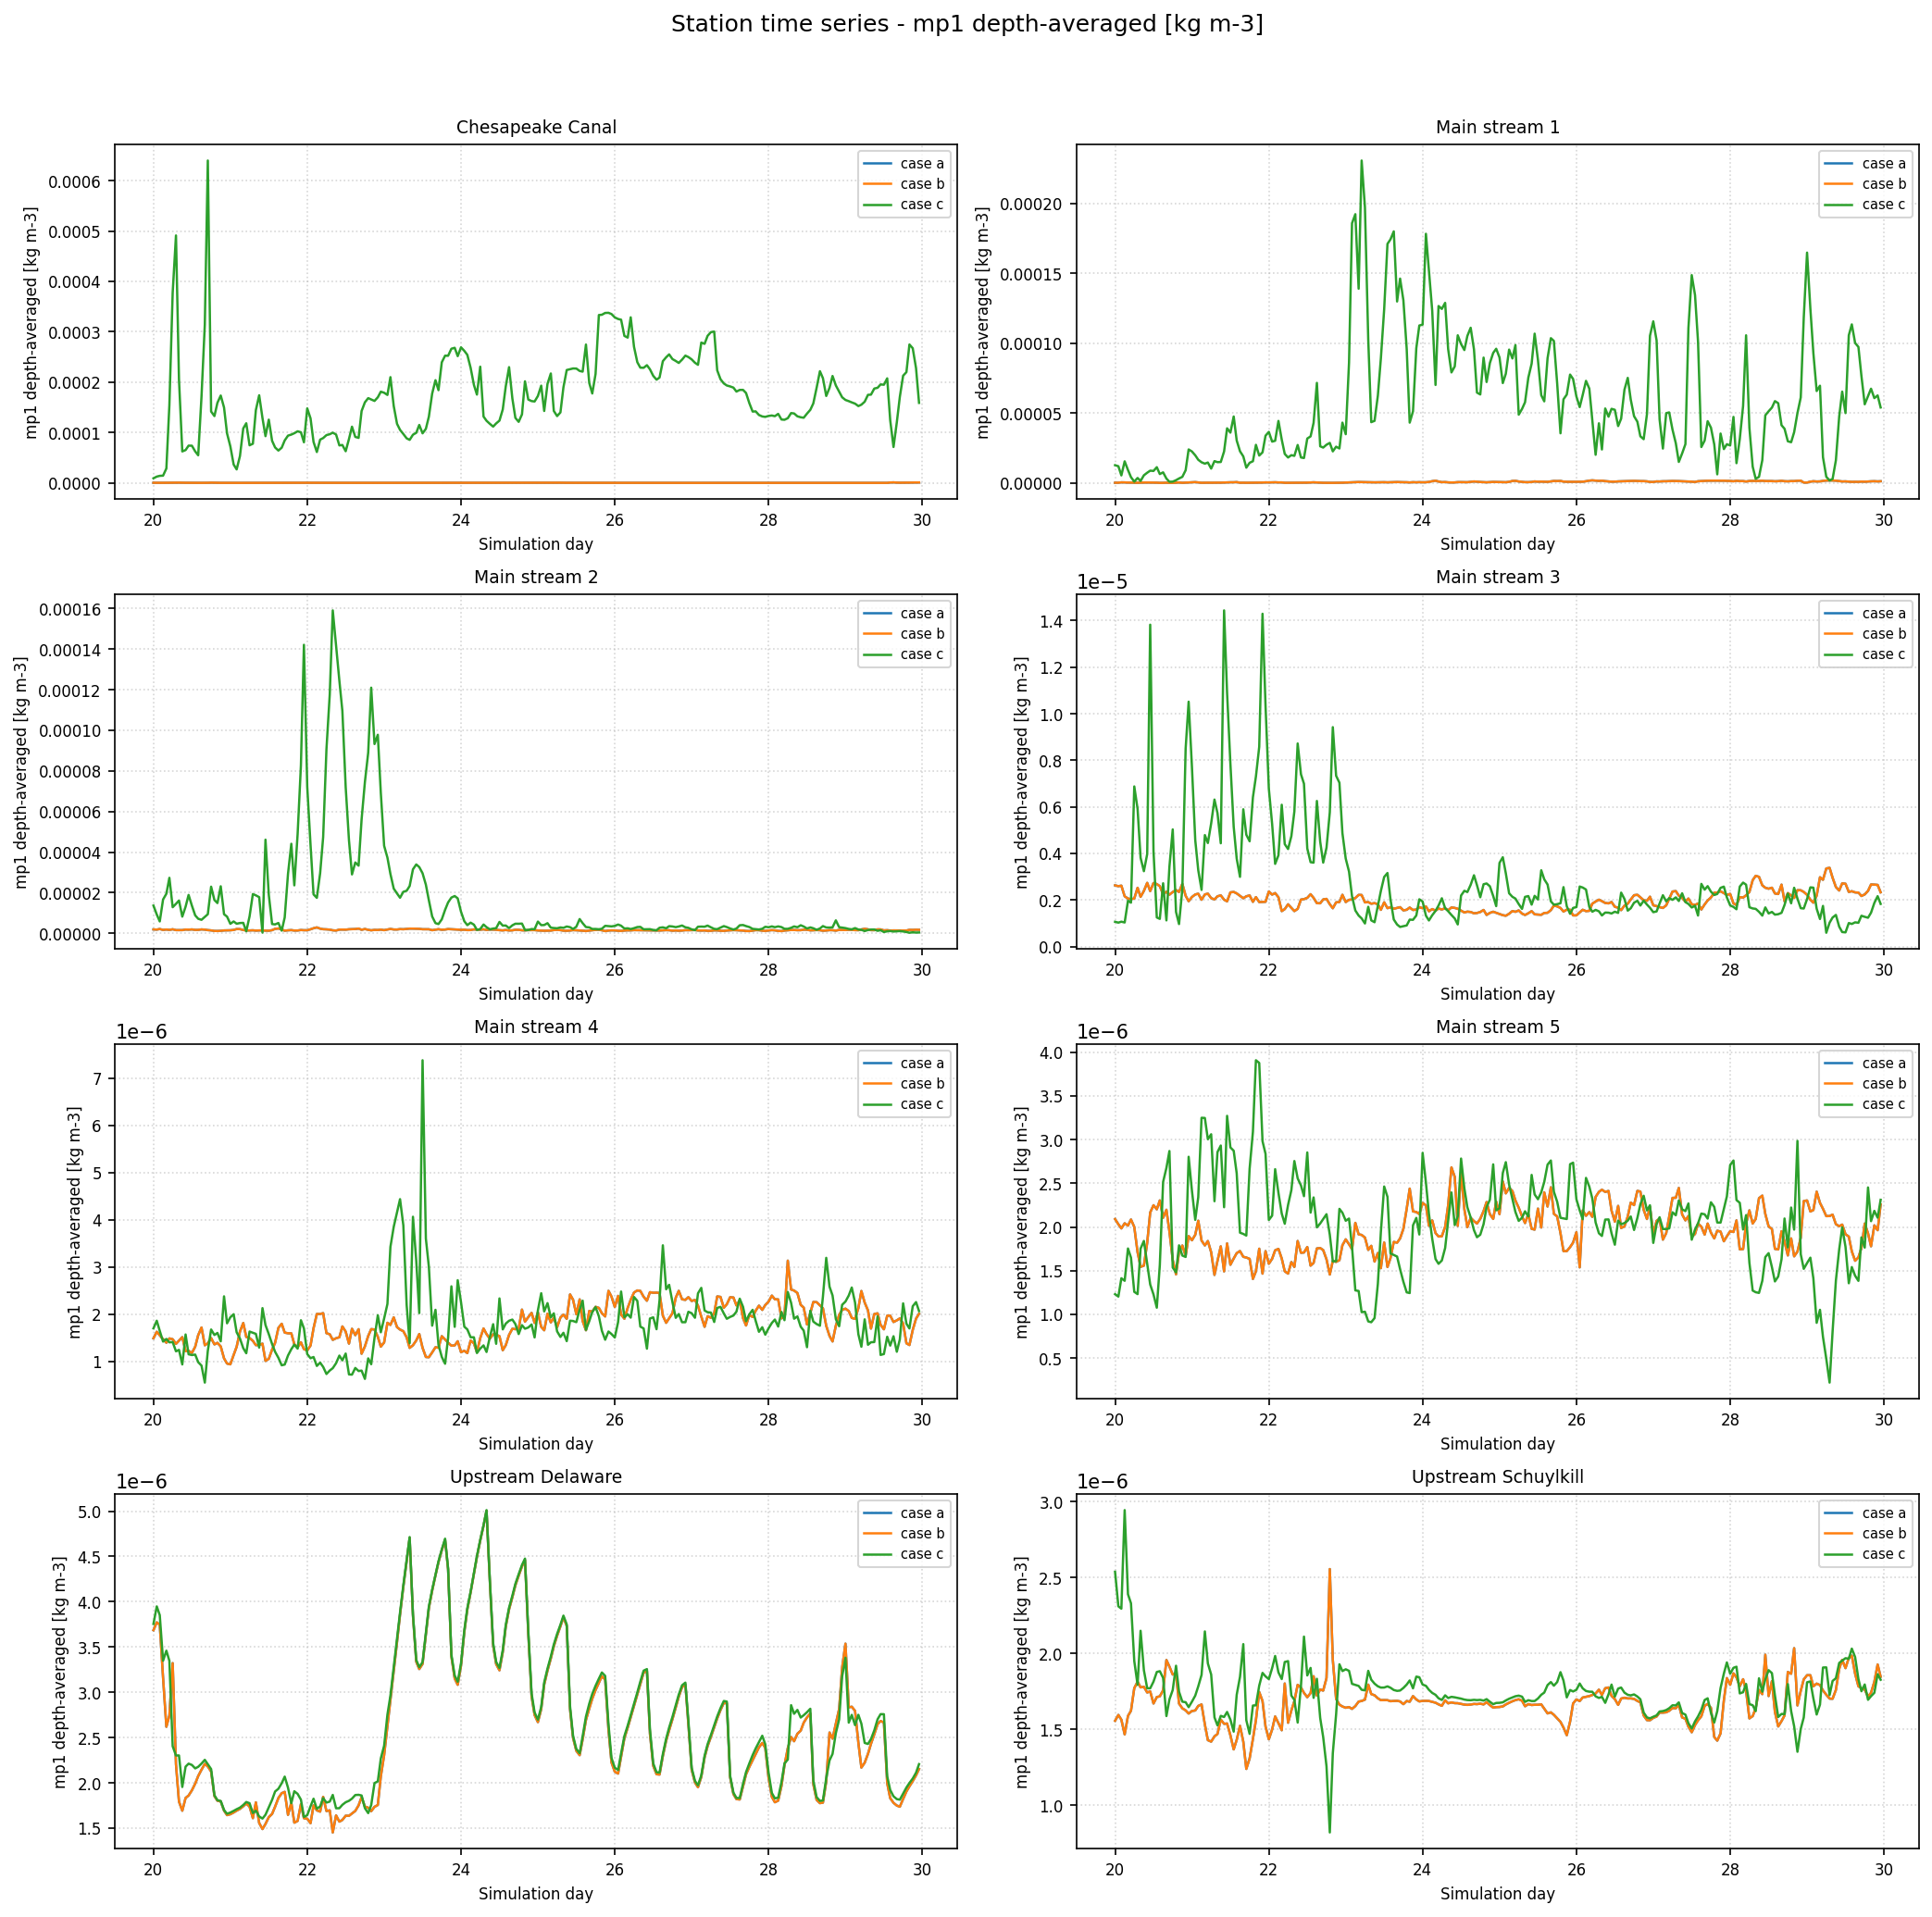
\includegraphics[width=\textwidth]{../FVCOM_MP_test_run/PYTHON/output/spatial_distribution/day30/station_timeseries_mp1_davg.png}
\caption{Depth-averaged \texttt{mp1} station time series for simulation days
         20.000--29.957.}
\label{fig:station_day30}
\end{figure}

\begin{figure}[H]
\centering
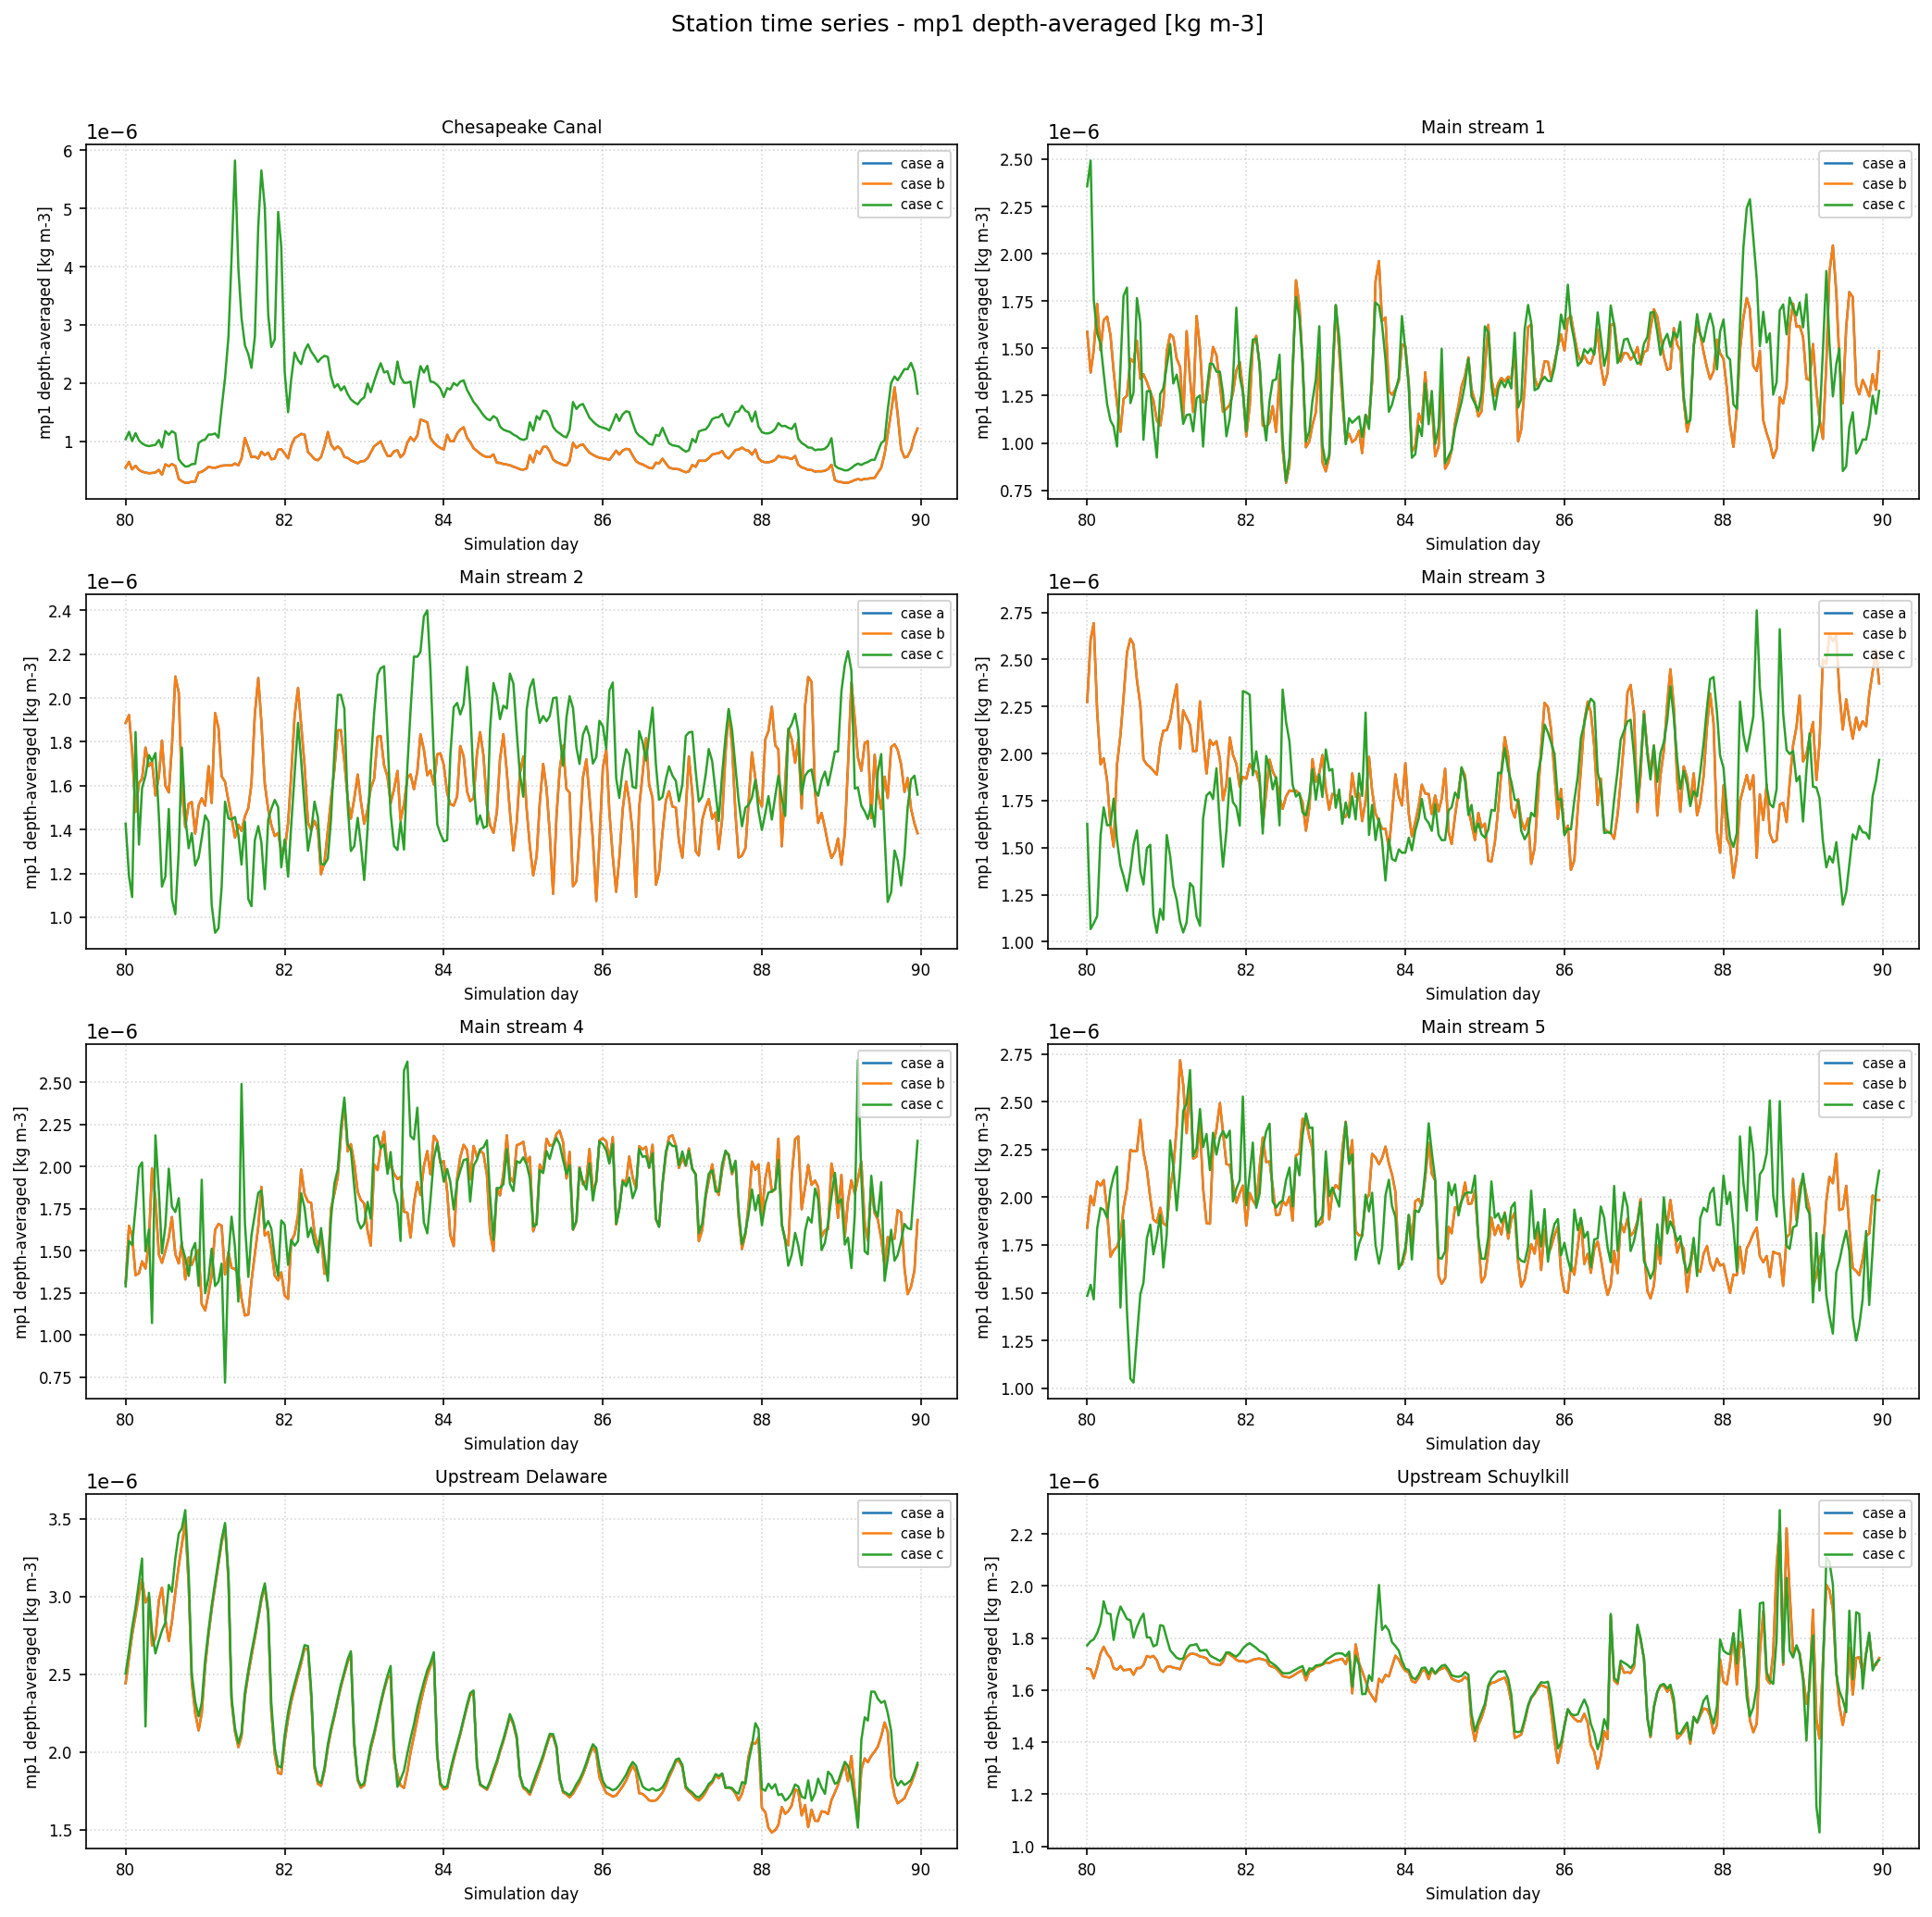
\includegraphics[width=\textwidth]{../FVCOM_MP_test_run/PYTHON/output/spatial_distribution/day90/station_timeseries_mp1_davg.png}
\caption{Depth-averaged \texttt{mp1} station time series for simulation days
         80.000--89.957.}
\label{fig:station_day90}
\end{figure}

\FloatBarrier

\section*{Observations}

\begin{enumerate}[(1)]
  \item \textbf{Cases a and b remain identical.}
        The late-time \texttt{b-a} differences are zero for
        depth-averaged \texttt{mp1} and bed mass in both windows.  This
        matches Memo~05: with the current fine-sediment parameterisation,
        case~\texttt{b} does not activate measurable aggregation or bed
        deposition.

  \item \textbf{Case c remains the active floc-interaction case.}
        At day~30, case~\texttt{c} has a day-mean depth-averaged
        \texttt{mp1} maximum of $4.62\times10^{-3}$~kg\,m$^{-3}$ and an
        aggregated-component maximum of $1.10\times10^{-3}$~kg\,m$^{-3}$.
        At day~90 those maxima are lower in the selected window
        ($1.49\times10^{-3}$ and $6.46\times10^{-5}$~kg\,m$^{-3}$,
        respectively) but the aggregated component remains positive across
        nearly the full domain.

  \item \textbf{Bed mass is present only in case c.}
        Cases~\texttt{a} and \texttt{b} remain zero-bed-mass runs.  In
        case~\texttt{c}, the day~30 window contains a large local bed-mass
        maximum ($1.95\times10^{-1}$~kg\,m$^{-2}$), while the day~90
        window has a smaller maximum ($2.21\times10^{-3}$~kg\,m$^{-2}$)
        but positive day-mean bed mass at almost all wet nodes.

  \item \textbf{No detached numerical hot spots are evident.}
        The pointwise-maximum maps retain coherent plume and near-source
        structures.  The maxima do not appear as isolated one-node artifacts
        disconnected from transport pathways.

  \item \textbf{Tracer split consistency remains tight.}
        The maximum depth-averaged split error in case~\texttt{c} remains
        below $5\times10^{-10}$~kg\,m$^{-3}$ in both late-time windows.
        This supports the interpretation that the late-time differences are
        physical/model-configuration differences rather than bookkeeping
        drift between total, aggregated, and disaggregated tracers.
\end{enumerate}

\section*{Summary}

The day~30 and day~90 spatial diagnostics support the Memo~05 conclusions at
later times.  Case~\texttt{a} and case~\texttt{b} remain numerically identical
under the present fine-sediment floc parameterisation.  Corrected
case~\texttt{c} continues to show active aggregation, disaggregated-water-column
transport, and bed exchange.  The late-time fields remain spatially coherent,
and the \texttt{mp1\_agg}+\texttt{mp1\_dis} consistency error remains at
roundoff-level magnitude.

\end{document}
